\documentclass[journal]{IEEEtran}
\usepackage[T1]{fontenc}
\usepackage{amsmath,amssymb}
\usepackage{graphicx}
\usepackage{booktabs}
\usepackage{multirow}
\usepackage{placeins}
\usepackage{float}
\usepackage{array}
\usepackage{xcolor}
\usepackage{tikz}

\usetikzlibrary{arrows.meta,positioning,fit,calc,backgrounds}
\usepackage[hidelinks]{hyperref}
\usepackage{cite}
\usepackage{url}

\definecolor{elblue}{HTML}{2A78D6}
\definecolor{foorange}{HTML}{EB6834}
\definecolor{rgreen}{HTML}{1BAF7A}
\definecolor{inkgray}{HTML}{52514E}
\newcommand{\best}[1]{\textbf{#1}}
\newcommand{\ms}{\,mph}
\definecolor{revisionblue}{HTML}{004AC2}
\newif\ifshowchanges
\showchangesfalse
\ifdefined\highlightchanges\showchangestrue\fi
\newcommand{\rev}[1]{\ifshowchanges{\color{revisionblue}\ifmmode\boldsymbol{#1}\else\bfseries\boldmath #1\fi}\else #1\fi}
\newcommand{\prev}[1]{#1}
\renewcommand{\dbltopfraction}{0.85}
\renewcommand{\topfraction}{0.85}
\renewcommand{\textfraction}{0.1}
\renewcommand{\dblfloatpagefraction}{0.8}
\setcounter{dbltopnumber}{3}

\newfloat{algorithm}{t}{loa}
\floatname{algorithm}{Algorithm}

\begin{document}

\title{Sparse Sensor Links for Low-Speed Traffic Forecasting: An Evaluation of Predictive Gain and Effective Resistance}

\author{Al~Zahraa~Altayasinah and Mohammed~Alawadhi%
\thanks{The authors are with the American University of Sharjah, Sharjah, United Arab Emirates. This report was prepared for MLR~570 Advanced Machine Learning. The project was originally titled ``Express Links: Targeted Graph Rewiring to Forecast Jams Across Traffic Bottlenecks.''}}

\markboth{MLR 570 Advanced Machine Learning, Final Project Report, November 2026}{Altayasinah and Alawadhi: Sparse Sensor Links for Low-Speed Traffic Forecasting}

\maketitle


\begin{abstract}
We study how adding sensor links affects hour-ahead forecasts of low traffic speeds on METR-LA and PEMS-BAY. \prev{Across 42 Graph WaveNet runs, we evaluated a greedy selector that scores each candidate link by multiplying its lead--lag correlation by its reduction in total effective resistance.} The selector lowered overall 60-minute mean absolute error (MAE) by 0.014 mph on METR-LA and 0.013 mph on PEMS-BAY. We then compared six graphs in 36 runs. \prev{Two of them chose links with the same simple linear (ridge) forecast of each road: Express Links first shortlisted poorly connected sources, while Forecast-only shortlisted the sources that most improved that forecast. Forecast-only gave} the lowest mean MAE on low-speed readings at the shared evaluation roads. It reduced MAE from 7.969 to 7.695 mph on METR-LA and from 5.223 to 5.127 mph on PEMS-BAY. On METR-LA it beat matched random links on all three seeds with both Graph WaveNet and DCRNN. A global virtual node gave the lowest network-wide 60-minute MAE in the six-way comparison. A five-seed test favored the original Forecast-only configuration over the tuned version on the primary metric. \prev{Neither of our two tests of whether the models actually used the added source roads met its decision rule,} so the contribution of over-squashing to these forecasting gains remains uncertain. \rev{The code, results and decision records are available at \url{https://github.com/alzahraa77/express-links-mlr570}.}
\end{abstract}

\begin{IEEEkeywords}
Traffic forecasting, spatio-temporal graph neural networks, graph rewiring, over-squashing, effective resistance, Graph WaveNet, DCRNN, pre-registration.
\end{IEEEkeywords}

%======================================================================
\section{Introduction}\label{sec:introduction}

\prev{\IEEEPARstart{T}{raffic} forecasting estimates future road conditions from historical sensor observations. Its practical relevance is illustrated by the deployment of graph neural networks for travel-time estimation \cite{derrowpinion2021eta}. The forecasting task requires a model to capture both temporal changes at individual sensors and spatial dependencies across the road network. DCRNN models these dependencies through bidirectional graph diffusion and recurrent sequence prediction \cite{li2018dcrnn}, while STGCN combines graph and temporal convolutions \cite{yu2018stgcn}. Graph WaveNet uses dilated temporal convolutions and a learned adaptive adjacency \cite{wu2019graphwavenet}. These architectures build on graph convolution and message passing \cite{kipf2017gcn,gilmer2017mpnn}, but their ability to use distant information depends on how sensors communicate.}

\prev{The physical road graph does not necessarily contain every dependency useful for forecasting. MTGNN learns directed relationships between time series \cite{wu2020mtgnn}, GTS learns a distribution over discrete graphs \cite{shang2021gts}, and AGCRN learns node-specific parameters and adaptive connectivity \cite{bai2020agcrn}. Attention-based approaches provide other ways to model spatial and temporal dependencies, including ASTGCN and GMAN \cite{guo2019astgcn,zheng2020gman}. PDFormer explicitly accounts for propagation delays and short- and long-range spatial relationships \cite{jiang2023pdformer}. These studies motivate examining which additional connections are useful, rather than assuming that greater connectivity will improve every forecast.}

\prev{A related concern is over-squashing: information from many nodes can be compressed into fixed-size representations as it passes through graph bottlenecks \cite{alon2021bottleneck}. Prior work relates this limitation to curvature \cite{topping2022curvature}, network width, depth and topology \cite{digiovanni2023oversquashing}, and effective resistance \cite{black2023resistance}, \prev{which is high when two nodes are joined only through a few long or narrow paths}. Rewiring methods therefore modify graph connectivity using criteria such as spectral expansion or locality \cite{karhadkar2023fosr,barbero2024laser}. Marisca et al. extend the analysis to spatiotemporal GNNs, where both spatial and temporal paths affect information propagation \cite{marisca2025stoversquashing}. Virtual nodes offer another communication route by connecting sensors through shared hubs \cite{cai2023mpnnvn,cao2025virtual}. However, these connections still need to carry information relevant to the forecasting task.} \prev{Fig.~\ref{fig:bottleneck} illustrates the idea: without an added link, information from a distant sensor must share one bottleneck road with everything else on its side of the network, whereas a direct link reaches the target in one hop. \prev{In the example in Fig.~\ref{fig:bottleneck}, which is for illustration only and is not taken from a dataset, road $u$'s information needs seven hops to reach road $v$, while one added link delivers it in a single hop. This is the mechanism we set out to test. Our diagnostics in Section~\ref{sec:results} did not show that it explains the gains we observed.}}

\begin{figure*}[!t]
\centering
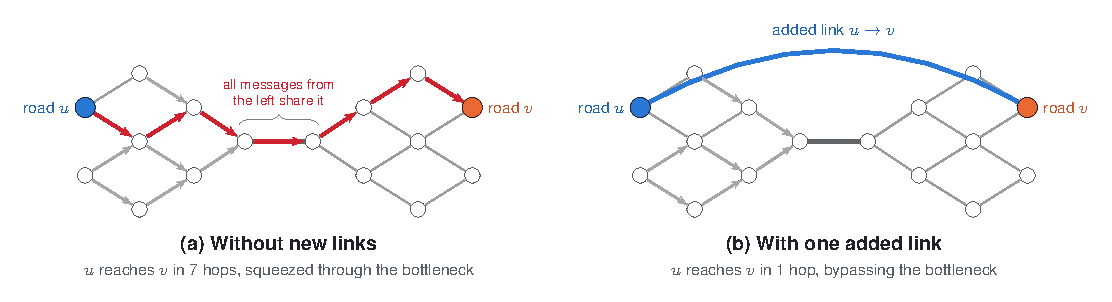
\includegraphics[width=0.78\textwidth]{figs/bottleneck_motivation.pdf}
\caption{\prev{Motivating example: an added link lets road $u$ reach road $v$ without passing through the bottleneck.}}
\label{fig:bottleneck}
\end{figure*}

\prev{Our motivation is the difficulty of hour-ahead forecasting under low-speed conditions. In our METR-LA baseline, mean absolute error (MAE) in the lowest speed band was more than twice the error across all readings. A slowdown at one sensor may provide early warning for another several hops away, suggesting that direct sensor links could make useful information more accessible. This leads to two questions: can a small number of added links improve low-speed forecasts, and does combining graph-connectivity information with predictive evidence help more than selecting links from predictive evidence alone? We distinguish these forecasting questions from the separate question of whether the models show evidence of reduced over-squashing.}

\prev{To investigate these questions, we add a budget of 25 directed links to the original road graph before training the forecaster. The initial greedy selector combines directional lead--lag correlation, \prev{which measures how strongly a slowdown at one sensor is followed by a slowdown at another a few minutes later}, with the reduction in total effective resistance produced by each addition. A follow-up compares two ridge-based selectors with the same final ranking procedure: Express Links shortlists weakly connected sources using pairwise effective resistance, whereas Forecast-only shortlists sources using predictive gain. The shortlisted links are ranked on a later block of training data. This predictive screen is related to the use of additional past information in Granger-style forecasting \cite{granger1969}, but is used here to select links rather than establish causal relationships.}

\prev{Our contributions are as follows.}
\begin{itemize}
\item \prev{We develop and evaluate a greedy selector that combines directional lead--lag correlation with total effective-resistance reduction, and compare it with six reference graphs, including a same-district control matched on lead--lag strength.}
\item \prev{We compare resistance-based and predictive shortlists within a common ridge-screening procedure on METR-LA and PEMS-BAY using Graph WaveNet, and evaluate the same frozen METR-LA graphs with DCRNN.}
\item \prev{We assess reliance on the selected sources using two input-replacement diagnostics, and evaluate changes to link number, distance, weight and allocation through validation-based tuning and a five-seed final comparison.}
\end{itemize}

\prev{On METR-LA, Forecast-only beat matched random links on all three seeds with both Graph WaveNet and DCRNN for 60-minute low-speed forecasts at the shared evaluation roads. The global virtual node achieved the lowest network-wide MAE in the six-way comparison.}

\prev{The rest of this report is organized as follows. Section~\ref{sec:related} reviews related work. Section~\ref{sec:methods} describes the forecasting task, the two link selectors and the control graphs. Section~\ref{sec:setup} gives the data, models and evaluation protocol, and Section~\ref{sec:results} reports the results. Section~\ref{sec:discussion} discusses what the results show, Section~\ref{sec:limitations} covers limitations and future work, and Section~\ref{sec:conclusion} concludes.}


\section{Related Work}\label{sec:related}

\subsection{Spatiotemporal traffic forecasting}
\prev{Graph-based traffic forecasting models differ in how they combine spatial aggregation and temporal prediction. DCRNN uses bidirectional diffusion within a recurrent encoder--decoder \cite{li2018dcrnn}. STGCN uses a fully convolutional design \cite{yu2018stgcn}, while T-GCN combines graph convolution with gated recurrent units \cite{zhao2020tgcn}. Graph WaveNet combines diffusion-based spatial aggregation with dilated temporal convolutions and adaptive adjacency \cite{wu2019graphwavenet}. ASTGCN weights spatial and temporal dependencies through attention \cite{guo2019astgcn}, and GMAN uses spatial and temporal attention blocks with an encoder--decoder design \cite{zheng2020gman}. These methods establish different forecasting backbones; our study evaluates graph augmentation while holding the backbone fixed within each comparison.}

\prev{The contribution of the architecture should also be distinguished from the representation of sensor and time identities. STID shows that identity embeddings with a multilayer perceptron can form a competitive forecasting baseline \cite{shao2022stid}. STAEformer combines spatiotemporal adaptive embeddings with temporal and spatial Transformer layers \cite{liu2023staeformer}. We therefore treat improved forecasting accuracy as evidence about the evaluated predictor and graph together. It does not, by itself, identify an information-propagation mechanism.}

\subsection{Learning predictive sensor dependencies}
\prev{Several forecasters learn relationships that are not specified by the road graph. Graph WaveNet learns an adaptive dependency matrix from sensor embeddings \cite{wu2019graphwavenet}. MTGNN learns directed dependencies jointly with spatial and temporal processing \cite{wu2020mtgnn}. GTS optimizes a distribution over discrete graphs \cite{shang2021gts}, while AGCRN combines adaptive graph generation with node-specific parameter learning \cite{bai2020agcrn}. STFGNN constructs temporal relationships from similarities between traffic series and combines them with spatial structure \cite{li2021stfgnn}. These approaches demonstrate that informative sensor relationships can extend beyond geographical adjacency.}

\prev{Our selectors also use traffic observations, but construct a fixed set of links before training the neural forecaster. The original road graph is retained, and the main sparse comparisons use the same link budget. Graph WaveNet's adaptive adjacency is disabled in these comparisons so that the supplied graph determines its spatial supports. This design evaluates explicit link-selection rules within a common forecasting model; it does not compare against the full range of learned-graph architectures.}

\subsection{Over-squashing and structural rewiring}
\prev{Alon and Yahav identify the compression of growing graph neighbourhoods into fixed-size representations as a limitation of message passing \cite{alon2021bottleneck}. Topping et al. connect bottlenecks to graph curvature and propose curvature-based rewiring \cite{topping2022curvature}. Di Giovanni et al. analyse how width, depth and topology affect sensitivity to distant inputs \cite{digiovanni2023oversquashing}. Black et al. relate information propagation to effective resistance and propose Greedy Total Resistance (GTR) rewiring \cite{black2023resistance}. Effective resistance is also connected to random-walk commute times \cite{chandra1996resistance}. These results motivate resistance as a structural criterion, while leaving its forecasting value to be evaluated empirically.}

\prev{Other methods balance connectivity against different graph properties. FoSR adds edges using spectral expansion and distinguishes original from added connections through a relational architecture \cite{karhadkar2023fosr}. DiffWire uses differentiable layers motivated by commute time and spectral-gap optimization \cite{arnaiz2022diffwire}. Expander Graph Propagation uses a sparse expander as a communication structure \cite{deac2022egp}. LASER explicitly considers locality and sparsity alongside over-squashing \cite{barbero2024laser}. DRew changes multi-hop connectivity by layer and introduces distance-dependent delays \cite{gutteridge2023drew}. Graph Diffusion Convolution provides a broader graph-preprocessing perspective by sparsifying a generalized diffusion operator \cite{gasteiger2019diffusion}; it is relevant to changing communication neighbourhoods without being a traffic-specific over-squashing diagnostic.}

\prev{These methods do not use the same selection criteria or evaluation tasks. In particular, FoSR reports graph-classification experiments \cite{karhadkar2023fosr}, whereas our task is multi-horizon traffic-speed regression. The Long Range Graph Benchmark provides tasks for evaluating long-range dependencies \cite{dwivedi2022lrgb}. Such evaluations motivate testing distant information use, but their results cannot be assumed to transfer to low-speed traffic forecasting. In our experiments, GTR is a structural control; the other rewiring methods discussed here provide context and were not evaluated as forecasting baselines.}

\subsection{Spatiotemporal propagation, attention and virtual nodes}
\prev{Spatial graph structure is only one part of information propagation in a spatiotemporal model. Marisca et al. analyse sensitivity on joint spatial and temporal paths and compare temporal and spatial processing arrangements \cite{marisca2025stoversquashing}. This distinction matters because a useful source must be accessible at an informative time as well as at a useful location. Our lead--lag criterion addresses temporal ordering in the observed speeds, while our ridge screen evaluates one source summary for a 60-minute target. Neither criterion is a direct measurement of the neural model's spatiotemporal sensitivity.}

\prev{Global communication is also available through attention and hubs. Graphormer incorporates structural information into a Transformer \cite{ying2021graphormer}, and GraphGPS combines structural or positional encodings, local message passing and global attention \cite{rampasek2022gps}. For traffic, PDFormer models propagation delay and spatial relationships through attention \cite{jiang2023pdformer}. Cai et al. establish connections between message passing with virtual nodes and graph Transformers \cite{cai2023mpnnvn}. Cao et al. incorporate virtual nodes into STGCN using adaptive and semi-adaptive adjacency \cite{cao2025virtual}. Our virtual-node control follows the hub-connectivity idea, using one fixed global hub with neutral input. It is not a reproduction of Cao et al.'s learned semi-adaptive model, and its edge budget is larger than that of the sparse selectors.}

\subsection{Predictive screening and Granger-style construction}
\prev{Granger-style analysis asks whether the past of one series improves prediction of another after conditioning on the information already included \cite{granger1969}. STGC-GNNs uses spatiotemporal alignment and Granger testing to construct dependencies for traffic prediction \cite{he2022stgc}. ST-CGI jointly learns a predictive graph and autoregressive processes \cite{zhang2022stcgi}, while MSA-GCN incorporates Granger testing within a multistage graph-processing architecture \cite{feng2024msagcn}. These studies show that graph construction based on incremental predictive information is an established direction.}

\prev{Our ridge screen uses the same general predictive principle with a deliberately restricted feature set. A source is useful if adding its recent-speed summary reduces ranking-block MAE beyond a target's own history, neighbourhood speed and time of day. We do not perform a formal Granger significance test or infer physical causation. The comparison instead asks whether a resistance-based shortlist improves link selection when the downstream predictive screen is held fixed.}

\subsection{Position of this study}
\prev{Our study combines structural and predictive link-selection criteria within a fixed forecasting protocol. The initial greedy rule weights total-resistance reduction by directional lead--lag correlation. The ridge-based comparison then changes only the shortlist criterion while retaining the final ranking procedure. Matched random links and GTR test alternative placement rules, and a global hub provides a different communication structure. Input replacement examines source reliance separately from predictive accuracy. Table~\ref{tab:literature_position} summarizes the closest methodological relationships. This positions the work as an empirical study of explicit sensor-link selection, with over-squashing as a motivation whose role must be assessed through additional evidence.}

\begin{table*}[!t]
\centering
\caption{\prev{Representative approaches and their relation to this study. Literature comparisons describe published designs; they do not indicate that every method was implemented as a baseline.}}
\label{tab:literature_position}
\footnotesize
\setlength{\tabcolsep}{4pt}
\begin{tabular}{@{}p{3.1cm}p{5.0cm}p{8.0cm}@{}}
\toprule
\prev{Approach} & \prev{Communication or selection principle} & \prev{Relationship to this study} \\
\midrule
\prev{Learned graphs \cite{wu2019graphwavenet,wu2020mtgnn,shang2021gts,bai2020agcrn}} & \prev{Infer sensor relationships during forecasting-model training} & \prev{Our links are selected in advance. Graph WaveNet with adaptive adjacency disabled is the main backbone; the other architectures provide context.} \\
\prev{GTR \cite{black2023resistance}} & \prev{Greedily reduce total effective resistance} & \prev{Implemented structural control. Our initial selector also uses directional lead--lag correlation.} \\
\prev{FoSR and LASER \cite{karhadkar2023fosr,barbero2024laser}} & \prev{Improve spectral connectivity or balance connectivity, locality and sparsity} & \prev{Context for structural rewiring. Our selectors additionally use traffic observations and target low-speed regression.} \\
\prev{DRew \cite{gutteridge2023drew}} & \prev{Layer-dependent multi-hop aggregation with delays} & \prev{Context for distance-sensitive communication. Our augmentation is fixed across layers and training.} \\
\prev{STGC-GNNs and ST-CGI \cite{he2022stgc,zhang2022stcgi}} & \prev{Construct or learn predictive dependencies using Granger-style analysis} & \prev{Closest predictive-graph context. Our ridge screen ranks a fixed budget of additions and is not a formal causal test.} \\
\prev{Virtual nodes \cite{cao2025virtual}} & \prev{Learn hub connections using adaptive or semi-adaptive adjacency} & \prev{Inspiration for the implemented fixed global-hub control; its added-edge budget exceeds that of the sparse selectors.} \\
\prev{PDFormer and STAEformer \cite{jiang2023pdformer,liu2023staeformer}} & \prev{Use attention, propagation-delay modelling or adaptive embeddings} & \prev{Context for alternative traffic architectures. Our study keeps the backbone unchanged within each graph comparison.} \\
\prev{This study} & \prev{Combine resistance with lead--lag evidence, or compare resistance and predictive shortlists} & \prev{Evaluate frozen directed additions, architecture transfer, source-reliance diagnostics and validation-based tuning.} \\
\bottomrule
\end{tabular}
\end{table*}


%======================================================================
\section{Methodology}\label{sec:methods}
%======================================================================
\subsection{Forecasting task and notation}\label{sec:task}
\prev{Let $G=(V,E,A)$ be a directed sensor graph with $N=|V|$ nodes and weighted adjacency $A\in\mathbb{R}^{N\times N}$. Sensor $v$ records speed $s_v(t)$ every five minutes. Following the sequence-forecasting formulation used in traffic models \cite{li2018dcrnn,wu2019graphwavenet}, let $X_t\in\mathbb{R}^{12\times N}$ contain the last hour of speeds, $Y_t\in\mathbb{R}^{12\times N}$ contain the next hour, and $c_t$ denote the time-of-day input. For an augmented graph $A'$, the forecasting model is}
\begin{equation}
\prev{\widehat Y_t=f_\theta(X_t,c_t;A').}
\label{eq:forecast_map}
\end{equation}
\prev{The task is continuous speed regression. We report the 60-minute horizon ($h=12$) unless otherwise stated. The initial experiment also derives jam warnings from predicted speeds; the follow-up focuses on the error of observed low-speed readings. Graph augmentation changes $A'$ while keeping the forecasting architecture fixed within each comparison.}

\textit{Low-speed readings.} Let $\tau_1$ be the 25th percentile of observed training speeds (57.2\ms{} on METR-LA and 62.2\ms{} on PEMS-BAY). A test reading is \emph{low-speed}, or in Band~1, if it is observed and below $\tau_1$. Missing readings, stored as zeros, are never scored. For a set of roads $T$, the low-speed error at horizon $h$ is
\begin{equation}
\mathrm{MAE}^{\mathrm{low}}_{T}(h)=\frac{1}{|\mathcal{L}_T(h)|}\sum_{(t,v)\in\mathcal{L}_T(h)}\bigl\lvert\hat s_v(t{+}h)-s_v(t{+}h)\bigr\rvert ,
\label{eq:lowmae}
\end{equation}
where $\mathcal{L}_T(h)=\{(t,v): v\in T,\ 0<s_v(t{+}h)<\tau_1\}$ is the set of observed low-speed test readings at roads in $T$.
With $T=V$ this is the Band~1 error over all roads. For the six-way comparison, $T$ is fixed to the 25 roads receiving a ridge-based Express Links edge and is shared by all methods. Table~\ref{tab:notation} collects the symbols used in the rest of the paper.

\begin{table}[!t]
\centering
\caption{Notation.}
\label{tab:notation}
\footnotesize
\setlength{\tabcolsep}{3pt}
\begin{tabular}{@{}>{\raggedright\arraybackslash}p{0.2\columnwidth}>{\raggedright\arraybackslash}p{0.74\columnwidth}@{}}
\toprule
Symbol & Meaning \\
\midrule
$G=(V,E,A)$ & Directed road graph with $N=|V|$ sensors and weighted adjacency $A$ \\
$s_v(t)$, $\hat s_v(t)$ & Observed and forecast speed of sensor $v$ at step $t$ (5 min) \\
$h$ & Forecast horizon in steps; $h=12$ is 60 minutes \\
$\tau_1$, Band~1 & 25th percentile of training speeds; readings below it are low-speed \\
$T$, $\mathcal{L}_T(h)$ & Evaluation roads and their observed low-speed readings \\
$\bar A$ & Undirected surrogate of $A$ used for distances and resistance \\
$L$, $L^+$ & Graph Laplacian $D-\bar A$ and its pseudoinverse \\
$R(u,v)$ & Effective resistance between $u$ and $v$ \\
$\mathcal{R}(G)$ & Sum of pairwise effective resistances on the scored component \\
$\Delta\mathcal{R}(u,v)$ & Drop in $\mathcal{R}$ if an edge $u$--$v$ is added \\
$\rho_{uv}$ & Lead--lag strength: largest correlation of $u$'s residual speed with $v$'s 5--60 min later \\
$q_t(u,v)$ & Greedy score at round $t$, $\rho_{uv}\,\Delta\mathcal{R}(u,v)$ \\
$d(u,v)$ & Shortest-path distance in hops on $\bar A$ \\
$g(u\to v)$ & Held-out gain: drop in ranking-block 60-min ridge MAE of $v$ when $u$'s speed is added \\
$K$, $w$ & Link budget (25) and added-link weight (median positive off-diagonal weight of $A$) \\
$m$ & Shortlist size per target (16) \\
\bottomrule
\end{tabular}
\end{table}


\begin{figure*}[!t]
\centering
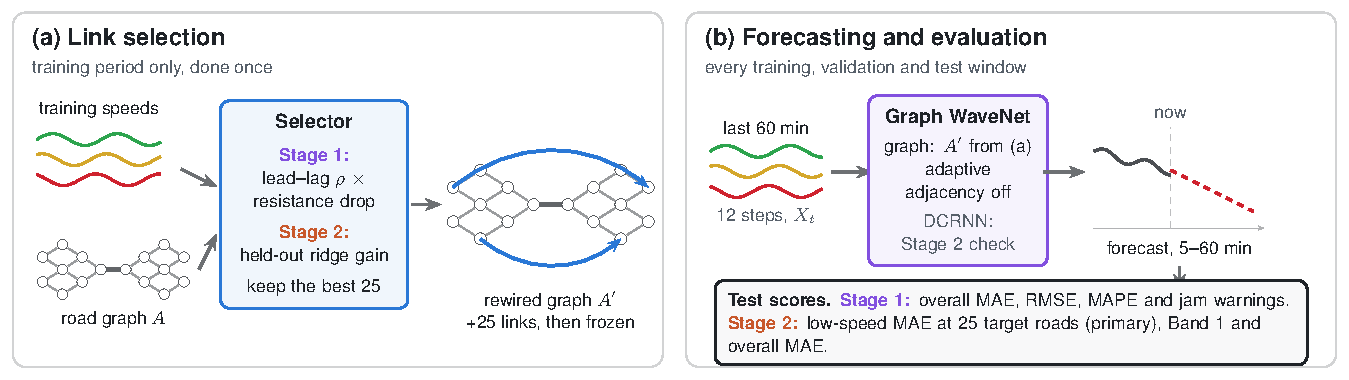
\includegraphics[width=0.95\textwidth]{figs/framework_overview.pdf}
\caption{\prev{Overview of the framework: links are chosen once from training data, and the forecaster is then trained on the frozen graph.}}
\label{fig:framework}
\end{figure*}

\begin{figure*}[!t]
\centering
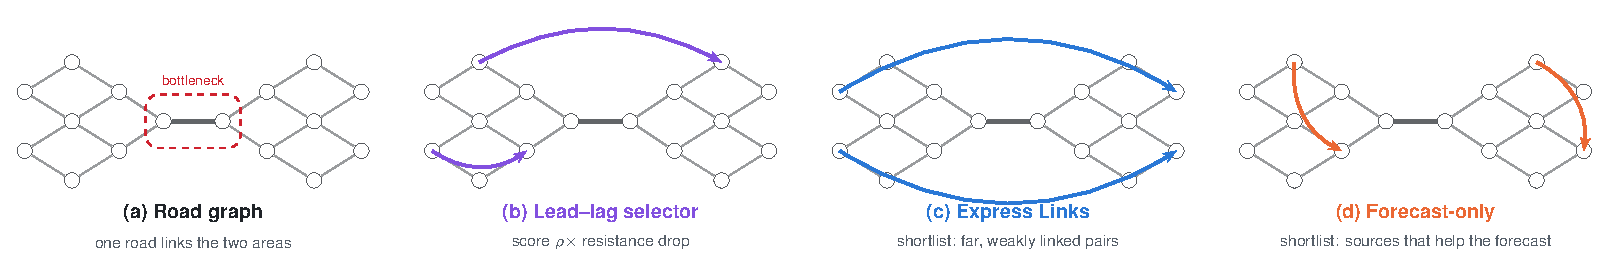
\includegraphics[width=\textwidth]{figs/selector_examples.pdf}
\caption{\prev{Kinds of links each selection rule tends to add, shown on a small example graph.}}
\label{fig:selector_examples}
\end{figure*}

\subsection{Framework overview}
\prev{The framework separates link construction from neural forecasting. A selector uses the road graph and training-period observations to choose a set $\mathcal B$ of additional directed sensor links. If $B_{uv}=1$ denotes a selected addition, the sparse augmented graph is}
\begin{equation}
\prev{A'=A+wB,\qquad B_{uv}\in\{0,1\},\quad \sum_{u,v}B_{uv}\leq K.}
\label{eq:augmentation}
\end{equation}
\prev{The default budget is $K=25$, and $w$ is the median positive off-diagonal weight of the original adjacency. Selected entries are absent from the original graph. The forecaster is then trained using the frozen augmented graph. These are computational communication links, rather than claims about new physical roads or causal influence.}

\prev{We evaluate two distinct selection procedures. The initial greedy procedure combines directional lead--lag evidence with the reduction in total effective resistance after each addition. The ridge-based follow-up first shortlists sources and then ranks their predictive value on a later training block. The follow-up compares a resistance-based shortlist with a predictive shortlist under the same final ranking. Their eligibility rules and symmetrization conventions are specified separately below. In the sparse Graph WaveNet comparisons, adaptive adjacency is disabled to keep the graph intervention explicit.}

\prev{Fig.~\ref{fig:framework} shows the whole pipeline in two parts. In part (a), link selection is done once, before any model is trained, using only training-period speeds and the road graph $A$. Stage~1 scores candidate pairs by lead--lag strength times the drop in total resistance, and Stage~2 scores them by held-out ridge gain. The best 25 links are added, and the resulting graph $A'$ is then frozen. In part (b), for every training, validation and test window, the forecaster receives the last 60 minutes of speeds from every sensor and uses $A'$ as its graph to predict the next 5 to 60 minutes. Graph WaveNet, with its adaptive adjacency switched off, is used in both stages, and DCRNN is a Stage~2 check. The box at the bottom of part (b) lists what we scored in each stage: overall MAE, RMSE, MAPE and jam warnings in Stage~1, and low-speed MAE at the 25 target roads, Band~1 MAE and overall MAE in Stage~2.}

\prev{Fig.~\ref{fig:selector_examples} shows, on a small example graph that is not taken from a dataset, the kind of links each rule tends to add (two links instead of 25). Panel (a) is the road graph, where a single road joins two areas. In panel (b), the Stage~1 lead--lag selector multiplies lead--lag strength by the resistance drop, so it can add links inside one area as well as across the bottleneck; on METR-LA only 3 of its 25 links crossed the bottleneck. In panel (c), Express Links shortlists distant, poorly connected pairs, so its links tend to be long. In panel (d), Forecast-only shortlists the sources that most improve the ridge objective on training data; on the real graphs these were closer to their targets and better connected on average (Fig.~\ref{fig:linkprops}).}


\subsection{Greedy lead--lag selector}\label{sec:greedy}
\prev{The first selector looks for pairs of roads where a slowdown at one road is reliably followed by a slowdown at the other, and favours pairs that the road graph connects poorly. To measure the first part, we remove each road's usual weekly pattern by subtracting its training-period median speed for that time of week, and standardize what is left. For an ordered pair $(u,v)$, the lead--lag strength $\rho_{uv}$ is the highest correlation between $u$'s adjusted speed and $v$'s adjusted speed 5 to 60 minutes later (lags of 1 to 12 steps). A high $\rho_{uv}$ means that changes at $u$ tend to show up at $v$ some minutes later. A pair is a candidate only if $u$ leads $v$ more strongly than $v$ leads $u$, the delayed correlation is higher than the same-time correlation, and $\rho_{uv}\geq0.2$. Both roads must be in the main connected part of the graph and must not already share a road link. We also skip dead ends, which are groups of at most three sensors attached to the rest of the graph by a single link.}

\prev{To measure the second part, we use effective resistance. Treat every road link as an electrical wire. The effective resistance $R(u,v)$ between two roads is low when many short routes join them and high when they are joined only through a few long or narrow routes, such as a single bridge. Adding a link between poorly connected roads lowers the total resistance $\mathcal{R}(G)$, summed over all pairs of roads, by a large amount. At round $t$, the selector multiplies the two parts:}
\[
\begin{aligned}
 q_t(u,v) &= \rho_{uv}\,[\mathcal{R}(G_t)-\mathcal{R}(G_t+uv)],\\
 \mathcal{R}(G_t) &= \sum_{i<j}R_{G_t}(i,j).
\end{aligned}
\]
\begin{algorithm}[!t]
\caption{Greedy lead--lag selector (Stage 1)}
\label{alg:greedy}
\small
\textbf{Input.} Road graph $A$, training speeds, link budget $K=25$.\par
\begin{enumerate}\setlength{\itemsep}{1pt}
\item Take the main component of $\max(A,A^\top)$ and compute $L^+$. Set $A'=A$ and choose $w$ as the median positive off-diagonal weight.
\item Remove the time-of-week median and standardize the residuals. For each pair, take the maximum correlation over lags 1--12. Keep eligible pairs that pass the lead--lag and dead-end criteria.
\item Repeat up to $K$ times while candidates remain. Choose the largest $q_t=\rho_{uv}\Delta\mathcal R(u,v)$ using Eq.~\eqref{eq:dR}. Set $A'_{uv}=w$ and compute $b=L^+(e_u-e_v)$. Update $L^+\leftarrow L^+ - wbb^\top/(1+wR(u,v))$ and remove both directions of the selected pair.
\end{enumerate}
\textbf{Output.} The augmented graph $A'$.
\end{algorithm}

\begin{figure}[!t]
\centering
\resizebox{\columnwidth}{!}{%
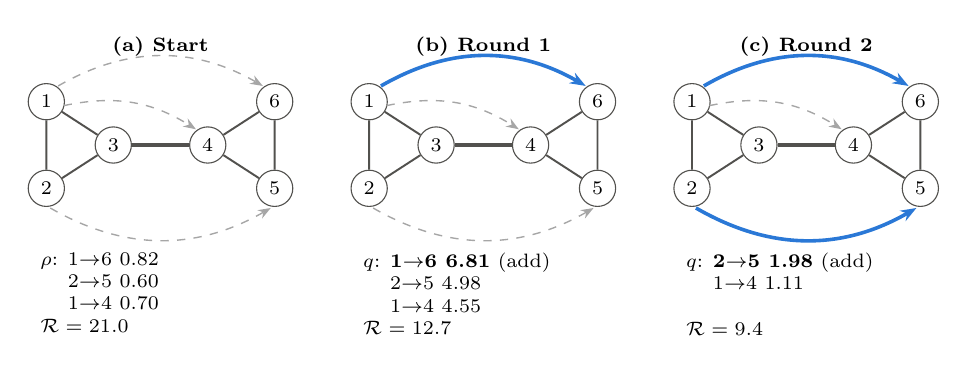
\begin{tikzpicture}[font=\footnotesize,
  nd/.style={circle, draw=inkgray, fill=white, inner sep=0pt, minimum size=4.6mm, font=\scriptsize},
  rd/.style={inkgray, line width=0.7pt},
  cand/.style={-{Stealth[length=1.6mm]}, dashed, gray!70, line width=0.5pt},
  new/.style={-{Stealth[length=2mm]}, elblue, line width=1.3pt}]
\foreach \dx/\lab in {0/(a) Start, 4.1/(b) Round 1, 8.2/(c) Round 2}{
  \begin{scope}[xshift=\dx cm]
  \node[nd] (n1) at (0,0.55) {1}; \node[nd] (n2) at (0,-0.55) {2}; \node[nd] (n3) at (0.85,0) {3};
  \node[nd] (n4) at (2.05,0) {4}; \node[nd] (n5) at (2.9,-0.55) {5}; \node[nd] (n6) at (2.9,0.55) {6};
  \draw[rd] (n1)--(n2)--(n3)--(n1); \draw[rd] (n4)--(n5)--(n6)--(n4); \draw[rd, line width=1.1pt] (n3)--(n4);
  \node[font=\scriptsize\bfseries] at (1.45,1.25) {\lab};
  \end{scope}}
% (a) candidates
\begin{scope}[xshift=0cm]
\draw[cand] (0.15,0.75) to[bend left=30] (2.75,0.75);
\draw[cand] (0.05,-0.8) to[bend right=30] (2.85,-0.8);
\draw[cand] (0.22,0.5) to[bend left=22] (1.9,0.2);
\end{scope}
% (b)
\begin{scope}[xshift=4.1cm]
\draw[new] (0.15,0.75) to[bend left=30] (2.75,0.75);
\draw[cand] (0.05,-0.8) to[bend right=30] (2.85,-0.8);
\draw[cand] (0.22,0.5) to[bend left=22] (1.9,0.2);
\end{scope}
% (c)
\begin{scope}[xshift=8.2cm]
\draw[new] (0.15,0.75) to[bend left=30] (2.75,0.75);
\draw[new] (0.05,-0.8) to[bend right=30] (2.85,-0.8);
\draw[cand] (0.22,0.5) to[bend left=22] (1.9,0.2);
\end{scope}
\node[align=left, font=\scriptsize, anchor=north west] at (-0.2,-1.25) {$\rho$: 1$\to$6 0.82\\\phantom{$\rho$: }2$\to$5 0.60\\\phantom{$\rho$: }1$\to$4 0.70\\$\mathcal{R}=21.0$};
\node[align=left, font=\scriptsize, anchor=north west] at (3.9,-1.25) {$q$: \textbf{1$\to$6 6.81} (add)\\\phantom{$q$: }2$\to$5 4.98\\\phantom{$q$: }1$\to$4 4.55\\$\mathcal{R}=12.7$};
\node[align=left, font=\scriptsize, anchor=north west] at (8.0,-1.25) {$q$: \textbf{2$\to$5 1.98} (add)\\\phantom{$q$: }1$\to$4 1.11\\[1.05em]$\mathcal{R}=9.4$};
\end{tikzpicture}}
\caption{\prev{Two rounds of the greedy lead--lag selector on a six-road example graph.}}
\label{fig:toy}
\end{figure}

\prev{Following the structural motivation of total-resistance rewiring \cite{black2023resistance}, we compute the resistance term on the undirected surrogate $\bar A=\max(A,A^\top)$. For a candidate edge of weight $w$, its reduction in total effective resistance is}
\begin{equation}
\Delta\mathcal{R}(u,v)=\frac{n_c\,w\,\lVert L^{+}(e_u-e_v)\rVert^2}{1+w\,R(u,v)},
\label{eq:dR}
\end{equation}
\prev{Here $n_c$ is the number of sensors in the main component, and $L^+$ is its Laplacian pseudoinverse. The calculation treats symmetrized edge weights as conductances \cite{spielman2011sparsification}. After selecting the highest-scoring candidate, we insert the directed link $u\to v$, apply the rank-one update to $L^+$, and recompute the structural scores. Thus, a link's score depends on the additions already made. Algorithm~\ref{alg:greedy} specifies the procedure. \prev{Fig.~\ref{fig:toy} works through two rounds on a six-road example: two triangles joined by one bridge, with every link given weight 1. The $\rho$ values in this example are chosen to show how the rule works; the resistance totals and scores are computed from the example graph. At the start, the total resistance is $\mathcal{R}=21.0$. In round 1, the scores $q=\rho\,\Delta\mathcal{R}$ are 6.81 for $1\to6$, 4.98 for $2\to5$ and 4.55 for $1\to4$, so $1\to6$ is added and $\mathcal{R}$ falls to 12.7. In round 2 the scores are recomputed: $1\to4$ has a higher $\rho$ than $2\to5$, but road 1 is now already well connected to road 4, so adding $1\to4$ would barely lower the resistance. Its score drops to 1.11, while $2\to5$ scores 1.98 and is added, leaving $\mathcal{R}=9.4$. This is why the scores are recomputed after every added link.} The structural calculation is undirected, while the inserted forecasting link retains its selected direction.}

\prev{To check how many selected links actually cross a bottleneck, we screened each road graph before training, using the road map only. We split the graph into regions at several resolutions and, for each region, compared the resistance between a road inside it and a road outside it with the resistance between two roads on the same side that are the same number of hops apart. A region counted as being behind a bottleneck if crossing into it cost at least as much extra resistance as in a reference layout of two street grids joined by only two crossings, and if this held at two or more resolutions and with both weighted and unweighted links. On METR-LA, one region passed: 9 sensors (4.4\%) sit behind three road links. PEMS-BAY had no region that passed, so it has no bottleneck subset. We call the areas separated by bottlenecks \emph{districts}; on PEMS-BAY all roads are in one district.}

\prev{The first comparison trains seven graphs on each dataset. Apart from the original road graph and the virtual node, every graph adds the same 25 directed links, so they differ only in where the links go:}
\begin{itemize}
\item \prev{\textbf{Original}: the road graph with no added links.}
\item \prev{\textbf{Lead--lag selector}: the greedy rule above, which scores each candidate by $\rho_{uv}$ times the drop in total resistance.}
\item \prev{\textbf{Random}: 25 pairs drawn at random from all eligible pairs, ignoring both lead--lag strength and resistance. It tests whether any extra links help.}
\item \prev{\textbf{Resistance only}: the same greedy loop scored by the drop in total resistance alone, ignoring lead--lag strength. It tests whether shortening long paths through the graph helps on its own.}
\item \prev{\textbf{Correlation only}: the 25 candidate pairs with the highest $\rho_{uv}$, ignoring resistance. It tests whether linking roads with related traffic helps on its own.}
\item \prev{\textbf{Same-side}: candidate pairs inside one district, each matched to the lead--lag strength of one selector link. On METR-LA it tests whether crossing the bottleneck matters when lead--lag strength is held equal; on PEMS-BAY, which has one district, it is simply a second set of strong lead--lag links.}
\item \prev{\textbf{Virtual node}: one extra node joined in both directions to every sensor, so any two sensors are at most two steps apart (414 added links on METR-LA). It adds far more links than the other graphs, so it is a reference for heavy extra connectivity rather than a matched control.}
\end{itemize}


\subsection{Candidate pairs and resistance-based screening}
\prev{The ridge-based follow-up uses $\bar A=(A+A^\top)/2$, with self-loops removed, for both shortest-path distances and effective resistance. Its eligible set is}
\begin{equation}
\prev{\mathcal C=\{(u,v):d_{\min}\leq d(u,v)<\infty,\ A_{uv}=0\},}
\label{eq:candidates}
\end{equation}
\prev{where $d(u,v)$ is unweighted hop distance on $\bar A$ and the default is $d_{\min}=3$. Tuning varies this minimum. The finite-distance condition prevents comparisons across disconnected components. Interpreting the weights of $\bar A$ as conductances \cite{klein1993resistance,spielman2011sparsification}, the pair resistance is}
\begin{equation}
R(u,v)=(e_u-e_v)^{\top}L^{+}(e_u-e_v).
\end{equation}
\prev{Here $L=D-\bar A$, $L^+$ is its pseudoinverse, and $e_u$ is the unit vector for node $u$. The eligibility rule gives 34{,}836 directed pairs on METR-LA and 90{,}400 on PEMS-BAY, with median distances of five and six hops, respectively. \prev{As in the first selector, high resistance means the two roads are poorly connected by the road graph.} High resistance identifies weakly connected pairs for the Express Links shortlist; it does not establish that their traffic signals will improve forecasts.}

\subsection{Training-only predictive screen}
\prev{Both follow-up selectors use ridge regression with $\alpha=1$ \cite{hoerl1970ridge}. To separate fitting from ranking, we split the training period chronologically into a fit block (first 80\% of training timestamps) and a ranking block (last 20\%). A window is assigned only when all of its forecast targets lie within the corresponding block; boundary-straddling windows are omitted. Each target must have at least 100 observed labels in both blocks. Neither validation nor test labels are used in this default link-ranking procedure.}

\prev{For target $v$, the base feature vector $x_v(t)$ contains its last 12 speeds, the weighted mean current speed of its neighbours in the symmetrized graph, and the sine and cosine of time of day. Missing inputs are forward-filled for at most three steps and then filled using fit-block medians. Standardization is fitted on the fit block. A candidate source $u$ contributes one additional feature, $z_u(t)$, equal to the mean of its last three speeds. The base and augmented ridge models are fitted on the fit block to predict $s_v(t+12)$.}

\prev{We evaluate the fitted models on the ranking block and define the held-out predictive gain as}
\begin{equation}
g(u\to v)=\mathrm{MAE}_{\mathrm{rank}}(\text{base})-\mathrm{MAE}_{\mathrm{rank}}(\text{base}+z_u).
\label{eq:predictive_gain}
\end{equation}
\prev{Positive gain means that the source summary improves prediction beyond the base features on this later training block. The screen follows the incremental-prediction principle associated with Granger-style analysis \cite{granger1969}; it is not a formal significance test and does not establish causal influence. It also evaluates a linear surrogate, so its ranking need not coincide with the eventual neural forecaster's ranking.}

\subsection{Shortlisting and final link selection}
\prev{The two ridge-based selectors differ in the shortlist supplied to the common ranking procedure (Fig.~\ref{fig:method}). For each target, at most $m=16$ eligible sources are retained:}
\begin{itemize}
\item \prev{\textbf{Express Links (EL)} keeps the 16 sources with the highest resistance $R(u,v)$ to the target, that is, the sources the road graph connects most poorly to it.}
\item \prev{\textbf{Forecast-only (FO)} keeps the 16 sources whose recent speed most improves the regularized ridge objective on the fit block. It never looks at resistance.}
\end{itemize}
\prev{Both selectors rank the shortlisted candidates by $g(u\to v)$. Each target retains its best positive-gain candidate, and the top $K=25$ candidates across targets are inserted with weight $w$ (0.320 on METR-LA). This gives at most one new link per target in the default configuration. We checked the transition-matrix convention so that an inserted $u\to v$ link passes the source signal toward the intended target in Graph WaveNet. The graph is then frozen before neural-model training.}

\prev{Algorithm~\ref{alg:ridge} specifies both variants. A common ranking rule does not guarantee common destinations: changing the shortlist can change both the selected sources and the targets receiving a link. The six-way evaluation therefore scores all models on the same set of 25 EL target roads, as defined in Section~\ref{sec:task}, while also reporting network-wide metrics.}

\prev{Fig.~\ref{fig:method} shows the two selectors step by step. On the left, the training period is split into a fit block (the first 80\%) and a ranking block (the last 20\%), and the road graph is made two-way ($\bar A$) to measure distance and resistance. A pair $u\to v$ is eligible if the two roads are at least three hops apart and not already linked. The dashed box is the only step where the selectors differ: for each target, Express Links keeps the 16 sources with the highest resistance $R(u,v)$, and Forecast-only keeps the 16 sources that most improve the regularized ridge objective on the fit block. Both then test each shortlisted source on the ranking block and keep it only if it lowers the error there ($g>0$). Each target keeps its best source, the 25 targets with the largest gains receive a link, and each link is given the usual road-link weight $w$. Graph WaveNet is then trained with these links on both datasets, and DCRNN on METR-LA.}

\begin{algorithm}[!t]
\caption{Ridge-based selectors: Express Links (EL) and Forecast-only (FO)}
\label{alg:ridge}
\small
\textbf{Input.} Road graph $A$, fit and ranking blocks, shortlist size $m=16$, link budget $K=25$, and selector.\par
\begin{enumerate}\setlength{\itemsep}{1pt}
\item Set $A'=A$. Compute distances and resistances on $(A+A^\top)/2$ without self-loops. Keep candidate pairs at finite distance of at least three hops with $A_{uv}=0$.
\item For each target with at least 100 observed labels in each block, fit the base ridge model on the fit block. Shortlist up to $m$ sources by pair resistance (EL) or improvement in the fit-block ridge objective (FO).
\item For each shortlisted source, evaluate the augmented fit-block model on the ranking block. Retain the best positive MAE gain per target.
\item Insert the top $K$ links by ranking-block gain, each with the median positive off-diagonal weight of $A$.
\end{enumerate}
\textbf{Output.} The augmented graph $A'$.
\end{algorithm}

\begin{figure*}[!t]
\centering
\resizebox{\textwidth}{!}{%
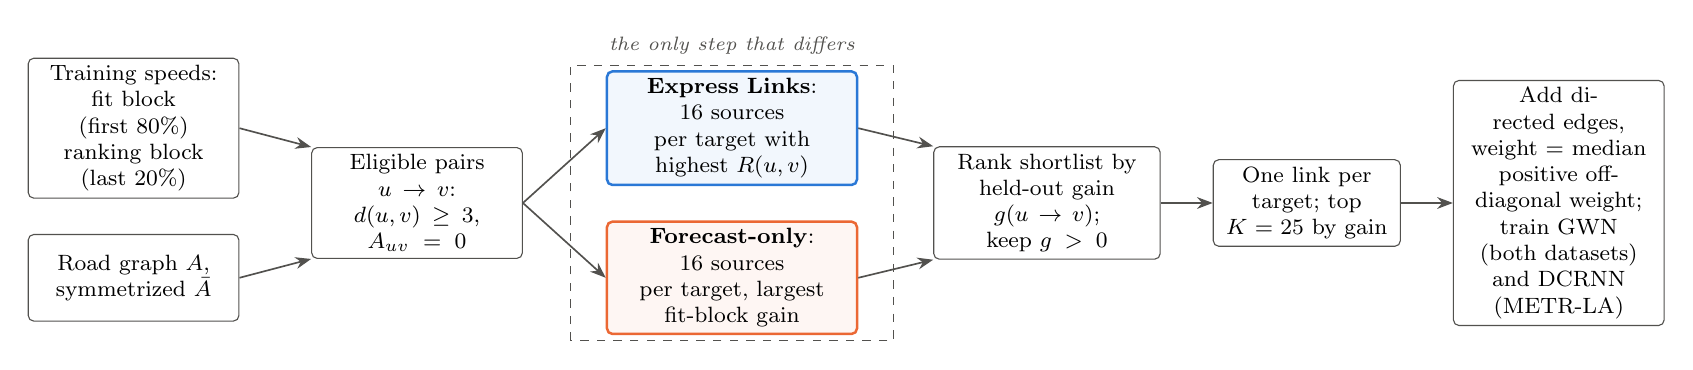
\begin{tikzpicture}[font=\footnotesize,
  box/.style={draw=inkgray, rounded corners=2pt, align=center, minimum height=11mm, inner sep=2.5pt, fill=white},
  el/.style={box, draw=elblue, line width=0.9pt, fill=elblue!6},
  fo/.style={box, draw=foorange, line width=0.9pt, fill=foorange!6},
  arr/.style={-{Stealth[length=2mm]}, inkgray, line width=0.6pt}]
\node[box, text width=25mm] (data) at (0,0.95) {Training speeds:\\fit block (first 80\%)\\ranking block (last 20\%)};
\node[box, text width=25mm] (graph) at (0,-0.95) {Road graph $A$,\\symmetrized $\bar A$};
\node[box, text width=25mm] (elig) at (3.6,0) {Eligible pairs $u\!\to\!v$:\\$d(u,v)\ge 3$, $A_{uv}=0$};
\node[el, text width=30mm] (elsl) at (7.6,0.95) {\textbf{Express Links}: 16 sources\\per target with highest $R(u,v)$};
\node[fo, text width=30mm] (fosl) at (7.6,-0.95) {\textbf{Forecast-only}: 16 sources\\per target, largest fit-block gain};
\node[box, text width=27mm] (rank) at (11.6,0) {Rank shortlist by\\held-out gain $g(u\!\to\!v)$;\\keep $g>0$};
\node[box, text width=22mm] (pick) at (14.9,0) {One link per\\target; top\\$K=25$ by gain};
\node[box, text width=25mm] (train) at (18.1,0) {Add directed edges,\\weight $=$ median\\positive off-diagonal weight;\\\prev{train GWN (both datasets)}\\\prev{and DCRNN (METR-LA)}};
\draw[arr] (data.east) -- (elig.north west);
\draw[arr] (graph.east) -- (elig.south west);
\draw[arr] (elig.east) -- (elsl.west);
\draw[arr] (elig.east) -- (fosl.west);
\draw[arr] (elsl.east) -- (rank.north west);
\draw[arr] (fosl.east) -- (rank.south west);
\draw[arr] (rank) -- (pick); \draw[arr] (pick) -- (train);
\draw[dashed, inkgray] (5.55,-1.75) rectangle (9.65,1.75);
\node[font=\scriptsize\itshape, text=inkgray] at (7.6,2.0) {the only step that differs};
\end{tikzpicture}}
\caption{\prev{The two ridge-based link selectors, Express Links and Forecast-only.}}
\label{fig:method}
\end{figure*}

\subsection{Control graphs}
\prev{The ridge-based comparison includes EL, FO and four reference graphs. The controls probe whether improvements depend on selected source locations, graph connectivity alone, or a global communication route:}
\begin{itemize}
\item \textbf{Original graph}: the road graph with no added links.
\item \textbf{Matched random}: 25 links into the same 25 target roads as Express Links, each from a uniformly random eligible source (fixed seed 0). This tests whether placement matters beyond adding a link to the same road.
\item \prev{\textbf{GTR}: 25 links chosen by Greedy Total Resistance rewiring \cite{black2023resistance}, which repeatedly adds the link that most lowers the total resistance of the graph. Each link is given one direction. It uses the road map only and no traffic data.}
\item \prev{\textbf{Virtual node}: one extra node that is not a real sensor, joined in both directions to every sensor (414 added links on METR-LA and 650 on PEMS-BAY). Any sensor can then pass information to any other in two steps, through this hub. The hub has no speed readings of its own, so we feed it zeros, and its forecasts are not scored. Cao et al.\ \cite{cao2025virtual} proposed virtual nodes for traffic with connections that the model learns; we use the simpler fixed version, where the hub links to everyone. Because it adds many more links than the 25 used by the other graphs, it is a reference rather than a matched control.}
\end{itemize}

\subsection{Diagnostics for information use}
\prev{A lower forecast error does not show \emph{why} a graph helped. To test whether the trained models actually use the added source roads, we run two diagnostics on the saved METR-LA Graph WaveNet models, without retraining. For a source--target pair, we replace the source road's last 12 speed readings with readings from another time and keep every other input the same. If the target's 60-minute error rises, the model was relying on the source's real readings. The size of that rise measures how much the model uses the source. The decision rules for both tests were written before we ran them. These tests measure use of a source; they cannot directly show that over-squashing was reduced.}

\textit{D1: week swap.} We replaced the source road's 12 input readings with readings from the same weekday and time in the nearest earlier training week with a complete record. If no complete record was available, we used the nearest earlier training week. We call the resulting change in the target's 60-minute MAE \emph{use}. A positive change means the actual source readings helped the model. We compared the extra use gained by adding Express Links ($A$) with the extra use gained by adding matched random links ($B$).
$A=\mathrm{Use}_{\mathrm{EL}}(\text{EL pairs})-\mathrm{Use}_{\mathrm{orig}}(\text{EL pairs})$, $B=\mathrm{Use}_{\mathrm{rand}}(\text{random pairs})-\mathrm{Use}_{\mathrm{orig}}(\text{random pairs})$, supported if $A-B>0$ with a 95\% day-bootstrap interval excluding zero on at least two of three seeds. The secondary rule asks whether the original model under-uses weakly connected sources, which is what over-squashing would predict. It matches candidate pairs with positive held-out ridge gain one-to-one, requiring the same hop distance, a gain difference of at most 20\% of the larger gain, and resistance on opposite sides of the median for that distance, and computes $C=\mathrm{Use}(\text{low-}R)-\mathrm{Use}(\text{high-}R)$, supported under the same seed and interval rule. A positive $C$ would mean the model uses well-connected sources more than equally useful, poorly connected ones. \prev{Intervals use 1{,}000 resamples of whole test days.}

\textit{D2: five matched donors.} \prev{For this test, we replaced} a source's 12 recent speeds with five histories from the validation period. The donor windows matched weekday or weekend status and were within 30 minutes of the original time of day. Among eligible windows, we chose those closest in the target's own recent speeds and neighbourhood speed. We measured the increase in MAE across the five replacements on low-speed target readings and called it \emph{reliance}. We used the same Express Links pairs and donors with all three models. To pass, the lower end of the paired 95\% day-bootstrap interval had to exceed $+0.01$\ms{} against both controls, with at least two of three seed estimates above $+0.01$\ms{} \prev{(10{,}000 bootstrap draws).} The high- versus low-resistance follow-up depended on passing this test.

\subsection{Tuning protocol}\label{sec:tuning-method}
We tuned Forecast-only on the METR-LA validation split. The primary metric was 60-minute Band~1 MAE across all roads, so every configuration was scored on the same readings even when the link budget changed. A configuration was eligible if its overall validation MAE was at most 0.01\ms{} above current Forecast-only (at least 3 hops between source and target, 25 links, and the standard link weight $w$, written $1\times$; $0.5\times$ and $2\times$ halve and double it). We chose the eligible configuration with the lowest Band~1 MAE if it improved by at least 0.02\ms{}. Otherwise we kept the current configuration. We fixed these rules before seeing the tuning results and locked the graphs and checkpoints before making test predictions. A tuned configuration passed on test if the upper 95\% day-bootstrap bound for its paired Band~1 difference was below zero against both current Forecast-only and its matched random control, and its overall MAE was at most 0.01\ms{} above current Forecast-only.

The search had three stages. The grid crossed minimum distance (3, 2 or 1 hops; one hop allows a reverse link to a directly connected road) with budget (10, 25, 50 or 100 links) at $1\times$ weight. The two best eligible grid set-ups were then retrained with $0.5\times$ and $2\times$ weight. Finally, an allocation stage compared two ways of giving up to three links per road at the winner's budget: by held-out gain, or to the roads where an original-graph model, trained on the first 80\% of training with preprocessing fitted on that period only, made the largest low-speed errors on the last 20\%. The error-based variant was adopted only if it beat both the winner and the gain-based allocation by 0.02\ms{}.

%======================================================================

\subsection{Computational considerations}
\prev{Link selection is performed offline. For a component with $n_c$ sensors, a dense Laplacian pseudoinverse requires quadratic storage and, under a standard dense decomposition, cubic initial computation. The greedy procedure then updates this matrix after each selected link instead of recomputing its pseudoinverse from scratch. Candidate screening can still involve a quadratic number of sensor pairs. The ridge procedure limits the later ranking to at most 16 sources per eligible target, although the predictive shortlist must first inspect the eligible candidates. These are properties of the procedure, not measured runtime improvements.}

\prev{At forecasting time, the sparse variants retain the original nodes and add at most $K$ adjacency entries; the virtual-node control adds one node and $2N$ directed links. Actual model runtime also depends on whether its support matrices are implemented densely or sparsely. A small edge budget therefore does not by itself establish a proportional training-time reduction.}

%======================================================================
\section{Experimental Setup}\label{sec:setup}
%======================================================================
\subsection{Data}
\prev{We use the two highway speed benchmarks released with DCRNN \cite{li2018dcrnn}. METR-LA covers 207 loop detectors on Los Angeles County highways over four months, and PEMS-BAY covers 325 detectors in the San Francisco Bay Area over six months. Each detector reports the average speed of passing vehicles every five minutes. METR-LA has 34{,}272 time steps, 1{,}515 road-graph edges and 8.109\% missing readings. PEMS-BAY has 52{,}116 steps after we removed 12 empty daylight-saving rows, 2{,}369 edges and 0.003\% missing readings. The road graph links sensors by driving distance along the network, so its edges are directed and weighted.}

\prev{Stage~1 downloaded the speed files from the authors' shared folder. By the time we set up Stage~2, that link no longer worked, so we took the speed files from the Torch Spatiotemporal research mirror \cite{cini2022tsl} and the road graphs from the official DCRNN repository. We recorded a checksum for every file and checked it at the start of each later step, so every Stage~2 experiment reads identical data.}

\subsection{Splits, missing data and normalization}
\prev{Both datasets use the standard chronological 70/10/20 split into training, validation and test periods. Stage~1 used the split from the Graph WaveNet code. It kept missing readings as zeros and masked them in the loss and the metrics. Stage~2 uses a stricter protocol. With the usual sliding windows, neighbouring splits share 11 target time steps, so we drop the windows that cross a boundary. This leaves 23{,}967, 3{,}417 and 6{,}843 training, validation and test windows on METR-LA, and 36{,}435, 5{,}201 and 10{,}412 on PEMS-BAY.}

\prev{In Stage~2, missing inputs are filled causally: a reading is carried forward for at most three steps, and any remaining gap takes that road's training median. Graph-based imputation can reconstruct missing readings \cite{cini2022grin}, but we keep the filling simple and score only observed labels, so no filled value is ever counted as a correct or wrong forecast. Inputs are standardized with the mean and standard deviation of the training windows. The speed-band thresholds are the training quartiles (57.2, 63.2 and 66.5\ms{} on METR-LA; 62.2, 65.3 and 67.5\ms{} on PEMS-BAY). The METR-LA test period has more missing readings than the training period (12.1\% against 7.1\%).}

\subsection{Models}
\prev{Graph WaveNet \cite{wu2019graphwavenet} is the forecaster in both stages. We use the official code at commit \texttt{6b162e80} with the adaptive adjacency switched off, so the model sees only the graph we give it. The other settings are the defaults of that code: double-transition supports, 32 hidden channels, diffusion order 2, dropout 0.3, Adam with learning rate $10^{-3}$ and weight decay $10^{-4}$, gradient clipping at 5 and batch size 64. Each run trains for 100 epochs, and we keep the checkpoint with the lowest validation MAE. In Stage~2, one training epoch took about 26 to 30 seconds on a single NVIDIA A10G GPU.}

\prev{DCRNN \cite{li2018dcrnn} is the second architecture, used only in Stage~2. We run the PyTorch implementation linked by the DCRNN project \cite{chnsh_dcrnn_pytorch} without changes: two recurrent layers of 64 units, diffusion order 2, and a sequence-to-sequence decoder trained with curriculum learning. It receives the same splits, frozen graphs and test readings as Graph WaveNet. It trains for up to 100 epochs and keeps the checkpoint with the lowest validation MAE.}

\prev{We trained DCRNN on METR-LA only, the same dataset we used for the diagnostics and the tuning study. A PEMS-BAY run was also planned, but only as a follow-up that depended on the tuning result. The plan was to use the tuned Forecast-only settings, choose new links from the PEMS-BAY training data, and train DCRNN with them, but only if the tuned version first passed its test on METR-LA. It did not pass (Section~\ref{sec:tuning}), so we did not run DCRNN on PEMS-BAY.}

\subsection{Seeds and common test readings}
\prev{Each graph is trained with several random seeds. We use seeds 0, 1 and 2 in Stage~1, the six-way comparison and the DCRNN transfer; seeds 0 and 1 while choosing tuning settings; and seeds 0 to 4 for the final tuning comparison. Within a dataset, every graph is scored on exactly the same test readings. We checked this with a fingerprint of the evaluation readings, which matched across graphs, seeds and both architectures on METR-LA.}

\subsection{Statistical evaluation}
\prev{Training noise from initialization and data order can be as large as the differences between graphs \cite{bouthillier2021variance}. For each comparison we therefore report the mean over seeds, the seed standard deviation and the number of seeds on which a graph beats its reference. Where we give confidence intervals, we use a paired day-block bootstrap \cite{efron1979,kunsch1989}. We resample whole test days with replacement, apply the same sampled days to both graphs and recompute the difference in MAE. Keeping each day intact preserves the strong correlation between readings taken minutes apart. The intervals use 1{,}000 resamples for the week-swap diagnostic and 10{,}000 for the five-donor diagnostic and the tuning test. For the DCRNN transfer we report paired seed comparisons only.}

\subsection{Protocol summary}
\prev{Table~\ref{tab:protocols} lists each experiment with its data, model, graphs, seeds, primary metric and decision rule. ``Low speed'' always means an observed reading below the training 25th-percentile speed (Band~1), and every error is a 60-minute MAE unless noted. Several decision rules were written down before the runs they govern \cite{nosek2018preregistration}, and the table marks these as pre-registered. One choice was not made in advance: we picked the primary metric for the six-way comparison, low-speed error at the 25 Express Links target roads, after looking at the seed-0 pilot, and fixed it before the replication runs.}

\begin{table*}[!t]
\centering
\caption{\prev{Experiments, models, metrics and decision rules (GWN = Graph WaveNet, EL = Express Links, FO = Forecast-only, VN = virtual node).}}
\label{tab:protocols}
\footnotesize
\begin{tabular}{@{}p{2.35cm}p{1.45cm}p{1.35cm}p{2.8cm}p{1.1cm}p{3.0cm}p{3.55cm}@{}}
\toprule
Experiment & Dataset & Model & Graphs & Seeds & Primary metric & Decision rule \\
\midrule
Stage 1 Lead--lag rewiring & METR-LA, PEMS-BAY & GWN & seven graphs & 0--2 & 60-min MAE and jam warnings & comparative evaluation \\
E1 Baseline reproduction & METR-LA, PEMS-BAY & GWN & road graph (paper split, strict split), full model & 0 & 12-horizon mean MAE vs. published & none \\
E2 Pilot & METR-LA & GWN & original, EL, FO, GTR, random, VN & 0 & exploratory & primary metric for E3 fixed after E2 \\
E3 Six-way replication & METR-LA, PEMS-BAY & GWN & original, EL, FO, GTR, random, VN & 0--2 & low-speed MAE at the 25 EL target roads & EL beats original and random on seeds 1 and 2 (pre-registered) \\
E4 Week-swap diagnostic (D1) & METR-LA & GWN (saved) & original, EL, random & 0--2 & added use of sources & $A-B>0$, interval excludes 0, $\ge$2/3 seeds (pre-registered) \\
E5 Five-donor diagnostic (D2) & METR-LA & GWN (saved) & original, EL, random & 0--2 & added reliance on EL sources, low-speed & lower 95\% bound $>{+}0.01$\ms{} vs. both, $\ge$2/3 seeds (pre-registered) \\
E6 Architecture transfer & METR-LA & DCRNN & original, EL, FO, random (frozen links) & 0--2 & as E3 & FO below random on $\ge$2/3 seeds and mean below original (pre-registered) \\
E7 FO tuning & METR-LA & GWN & FO variants, original, random & val.\ 0--1; final 0--4 & Band~1 MAE, all roads & Sec.~\ref{sec:tuning-method} (pre-registered, test plan locked) \\
\bottomrule
\end{tabular}
\end{table*}

%======================================================================
\section{Results}\label{sec:results}
%======================================================================
\subsection{Stage 1: the selector as proposed}\label{sec:stage1}

\prev{We first ran the greedy selector as proposed, against six reference graphs, with the Stage~1 pipeline. Each graph was trained with three seeds on both datasets, giving 42 Graph WaveNet runs. Table~\ref{tab:stage1} reports the 60-minute MAE and the average over all 12 horizons. Each entry is the mean over seeds, with the seed standard deviation in parentheses, and the lowest mean in each column is in bold. The greedy selector lowered overall 60-minute MAE by 0.014\ms{} on METR-LA and 0.013\ms{} on PEMS-BAY compared with the original graph. On METR-LA this gain is smaller than the selector's own seed standard deviation (0.028\ms{}). The virtual node, which connects to every sensor, had the lowest 60-minute error on METR-LA and tied with the greedy selector on PEMS-BAY. Averaged over all horizons, the greedy selector was best on PEMS-BAY.}

\begin{table}[!t]
\centering
\caption{\prev{Stage~1 results: Graph WaveNet MAE (mph) with each graph, mean (seed standard deviation) over seeds 0--2.}}
\label{tab:stage1}
\footnotesize
\setlength{\tabcolsep}{2pt}
\begin{tabular}{@{}lcccc@{}}
\toprule
& \multicolumn{2}{c}{METR-LA} & \multicolumn{2}{c}{PEMS-BAY} \\
\cmidrule(lr){2-3}\cmidrule(lr){4-5}
Graph & 60 min & 12-step mean & 60 min & 12-step mean \\
\midrule
Original & 3.582 (0.014) & 3.073 (0.001) & 1.964 (0.005) & 1.590 (0.006) \\
Random & 3.585 (0.014) & 3.080 (0.008) & 1.961 (0.007) & 1.587 (0.003) \\
Resistance only & 3.566 (0.016) & 3.063 (0.005) & 1.958 (0.006) & 1.588 (0.003) \\
Correlation only & 3.587 (0.002) & 3.081 (0.008) & 1.964 (0.001) & 1.589 (0.003) \\
Same-side & 3.586 (0.016) & 3.072 (0.010) & 1.962 (0.008) & 1.588 (0.005) \\
Lead--lag selector & 3.569 (0.028) & 3.069 (0.014) & \best{1.951} (0.002) & \best{1.582} (0.005) \\
Virtual node & \best{3.548} (0.020) & \best{3.058} (0.007) & \best{1.951} (0.012) & 1.588 (0.005) \\
\bottomrule
\end{tabular}
\end{table}

\prev{Fig.~\ref{fig:stageone} shows the same comparison seed by seed. Each point is the change in 60-minute MAE against the original graph at the same seed; the diamonds mark the three-seed means, and negative values favour the added links. Every difference lies within about 0.05\ms{} of zero. The greedy selector beat the original graph on two of three seeds on METR-LA and on all three on PEMS-BAY. Resistance-only links also helped on every seed of both datasets, though by at most 0.042\ms{}.}

\begin{figure*}[!t]
\centering
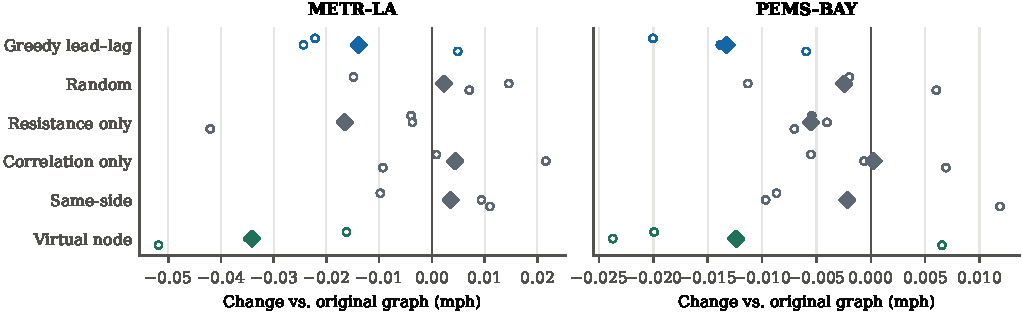
\includegraphics[width=.92\textwidth]{figs/stage_one.pdf}
\caption{\prev{Seed-level change in 60-minute MAE relative to the original graph for each Stage~1 graph.}}
\label{fig:stageone}
\end{figure*}

\prev{Fig.~\ref{fig:tradeoff} shows what each rule chose, by plotting the mean lead--lag strength of its 25 links against the drop in total effective resistance of the road graph. The virtual node is left out because it adds a hub node with a different link budget. Resistance-only links cut total resistance by 45.5\% on METR-LA and 38.4\% on PEMS-BAY, but their mean lead--lag correlations were only 0.03 and 0.10. Correlation-only links had the strongest correlations (0.51 and 0.58) and cut METR-LA resistance by just 6.4\%. The greedy selector sat between the two, with correlations of 0.28 and 0.47 and resistance reductions of 23.6\% and 36.2\%. A large drop in resistance did not guarantee better forecasts. On METR-LA, random links cut resistance by 36.1\% with a mean correlation of 0.08, yet overall 60-minute MAE rose slightly, from 3.582 to 3.585\ms{} (Table~\ref{tab:stage1}).}

\begin{figure}[!t]
\centering
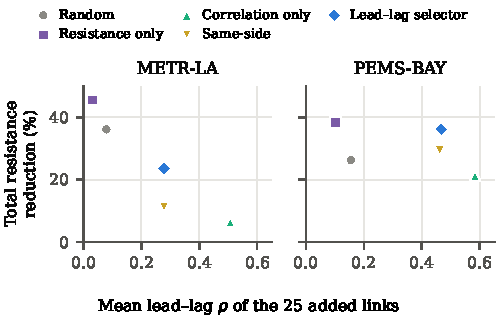
\includegraphics[width=\columnwidth]{figs/stage1_tradeoff.pdf}
\caption{\prev{Mean lead--lag strength of the 25 added links against the drop in total effective resistance, for each Stage~1 rule.}}
\label{fig:tradeoff}
\end{figure}

\prev{Only 3 of the 25 greedy links on METR-LA crossed the screened bottleneck boundary. To score jam warnings, we counted a jam onset when speed fell by at least 20\,km/h (about 12.4\ms{}) within 15 minutes, with a 15-minute persistence check where the horizon allowed it. A warning counted if it matched an observed onset within 15 minutes. At the 60-minute horizon, all seven graphs missed all 66 scored events behind the METR-LA bottleneck. Across all roads, mean recall ranged from 7.7\% to 9.1\% on METR-LA and from 1.5\% to 3.0\% on PEMS-BAY (Table~\ref{tab:events} in Appendix~\ref{app:other}). PEMS-BAY had no qualifying bottleneck subset. We also ran a gentler check that starts from events we know occurred and asks how close the forecast speed was. On PEMS-BAY, the share of events forecast within 10\ms{} of the observed speed was 51.7\% for the original graph, 53.1\% for the greedy selector and 54.6\% for the virtual node.}

\prev{Finally, we reran the METR-LA seed-0 models with causal input filling instead of zeros. The 60-minute MAEs were 3.520, 3.521 and 3.496\ms{} for the original, random and greedy graphs, so the greedy graph's advantage over random was 0.025\ms{}. Differences this small, together with the weak jam-warning results, motivated the regression-based follow-up in Stage~2.}

\subsection{E1: Baseline reproduction}
\prev{Before testing any added links, we checked that our Graph WaveNet baseline matched the published results. Table~\ref{tab:baseline} gives MAE, RMSE and MAPE averaged over the 12 horizons, and MAE at 15, 30 and 60 minutes. Published values come from the Graph WaveNet paper, and bold marks the best of our runs in each column. With the fixed road graph, our 12-horizon mean MAE was 3.070 against the published 3.08 on METR-LA, and 1.592 against 1.59 on PEMS-BAY. The full model with adaptive adjacency was slightly worse than published (3.071 against 3.04, and 1.589 against 1.58), with a larger gap at longer horizons. It reached a lower validation MAE, but we used the fixed graph in the follow-up so that we controlled exactly which links the model received. Our strict, causally filled baseline had the lowest mean MAE of our METR-LA runs and was about 0.003\ms{} above the fixed-graph run on PEMS-BAY.}

\begin{table}[!t]
\centering
\caption{\prev{Graph WaveNet reproduction against the published results (seed 0, 100 epochs).}}
\label{tab:baseline}
\footnotesize
\setlength{\tabcolsep}{3pt}
\begin{tabular}{@{}lcccc@{}}
\toprule
& 12-horizon mean & 15 min & 30 min & 60 min \\
\midrule
\multicolumn{5}{@{}l}{\textit{METR-LA}}\\
Paper, full model & 3.04 / 6.09 / 8.23 & 2.69 & 3.07 & 3.53 \\
Paper, fixed graph & 3.08 / 6.13 / 8.25 & -- & -- & -- \\
Ours, full model & 3.071 / 6.175 / 8.35 & 2.706 & 3.112 & 3.576 \\
Ours, fixed graph & 3.070 / 6.147 / \best{8.20} & 2.706 & 3.103 & 3.600 \\
Ours, strict (baseline) & \best{3.052} / \best{6.066} / 8.27 & \best{2.701} & \best{3.085} & \best{3.556} \\
\midrule
\multicolumn{5}{@{}l}{\textit{PEMS-BAY}}\\
Paper, full model & 1.58 / 3.52 / 3.55 & 1.30 & 1.63 & 1.95 \\
Paper, fixed graph & 1.59 / 3.55 / 3.57 & -- & -- & -- \\
Ours, full model & \best{1.589} / 3.562 / \best{3.56} & \best{1.305} & \best{1.646} & 1.978 \\
Ours, fixed graph & 1.592 / \best{3.550} / 3.64 & 1.317 & 1.650 & 1.975 \\
Ours, strict (baseline) & 1.595 / 3.558 / 3.57 & 1.319 & 1.657 & \best{1.973} \\
\bottomrule
\end{tabular}
\end{table}

\prev{The size of the error at low speeds is the main reason this study focuses on them. On METR-LA, the baseline's 60-minute MAE was 7.612\ms{} in Band~1, against 2.699, 1.919 and 1.563\ms{} in the three faster bands. A model that looks accurate overall can still be far off exactly when traffic slows down.}

\subsection{E2: Seed-0 pilot}
\prev{The METR-LA pilot trained each of the six graphs once, with seed 0. On the 30{,}331 low-speed readings at the 25 Express Links destinations, Forecast-only had the lowest 60-minute MAE (7.456\ms{}, against 7.603 for Express Links and 7.926 for the original graph). The virtual node was best overall (3.516\ms{}) but worse on those slow readings (8.174\ms{}). Rerunning the baseline with seed 0 gave an overall MAE of 3.553 instead of 3.556 and a best epoch of 91 instead of 80, a reminder of how much training noise there is. The pilot also showed how concentrated the Express Links graph was: just three source roads supplied all 25 links, and one of them supplied 18. Based on the pilot, we chose the target-road metric and fixed the decision rule before the replication.}

\subsection{E3: Six-way replication}
\prev{We then trained the six graphs on both datasets with three seeds each, for 36 runs under the strict protocol. All graphs were scored on the same 25 roads per dataset, with 30{,}331 low-speed readings on METR-LA and 77{,}284 on PEMS-BAY. Table~\ref{tab:sixway} gives four views of the 60-minute error: low-speed and all readings at the 25 target roads, and low-speed and all readings across the whole network. Each cell shows the mean over seeds, the seed standard deviation in parentheses, the change from the original graph, and in brackets the number of seeds on which the graph beat the original. Bold marks the best mean per dataset and column.}

\begin{table*}[!t]
\centering
\caption{\prev{Six-way Graph WaveNet comparison: 60-minute MAE (mph) over seeds 0--2.}}
\label{tab:sixway}
\footnotesize
\setlength{\tabcolsep}{3.5pt}
\resizebox{\textwidth}{!}{%
\begin{tabular}{@{}llllll@{}}
\toprule
Dataset & Graph & Low-speed, 25 target roads (primary) & All readings, 25 target roads & Low-speed, all roads (Band 1) & All readings, all roads \\
\midrule
\multirow{6}{*}{METR-LA}
& Original & 7.969 (0.040) & 3.136 (0.029) & 7.578 (0.075) & 3.554 (0.008) \\
& Express Links & 7.828 (0.230) $-$0.140 [2/3] & 3.141 (0.047) $+$0.006 [1/3] & 7.486 (0.062) $-$0.092 [2/3] & 3.541 (0.006) $-$0.013 [3/3] \\
& Forecast-only & \best{7.695} (0.291) $-$0.274 [2/3] & 3.169 (0.023) $+$0.033 [1/3] & \best{7.432} (0.100) $-$0.146 [3/3] & 3.564 (0.017) $+$0.010 [1/3] \\
& GTR & 8.181 (0.144) $+$0.213 [0/3] & 3.134 (0.018) $-$0.001 [1/3] & 7.615 (0.086) $+$0.037 [2/3] & 3.542 (0.018) $-$0.012 [3/3] \\
& Matched random & 8.058 (0.292) $+$0.089 [1/3] & 3.187 (0.077) $+$0.052 [0/3] & 7.546 (0.169) $-$0.032 [1/3] & 3.565 (0.020) $+$0.011 [1/3] \\
& Virtual node & 7.932 (0.242) $-$0.036 [2/3] & \best{3.105} (0.045) $-$0.030 [2/3] & 7.551 (0.230) $-$0.027 [1/3] & \best{3.522} (0.021) $-$0.032 [3/3] \\
\midrule
\multirow{6}{*}{PEMS-BAY}
& Original & 5.223 (0.039) & 2.338 (0.019) & 4.684 (0.040) & 1.968 (0.014) \\
& Express Links & 5.131 (0.023) $-$0.091 [3/3] & \best{2.305} (0.014) $-$0.033 [3/3] & 4.667 (0.058) $-$0.017 [2/3] & 1.963 (0.015) $-$0.005 [2/3] \\
& Forecast-only & \best{5.127} (0.160) $-$0.096 [2/3] & 2.314 (0.036) $-$0.024 [3/3] & 4.662 (0.065) $-$0.022 [2/3] & 1.964 (0.014) $-$0.004 [3/3] \\
& GTR & 5.158 (0.096) $-$0.065 [2/3] & 2.316 (0.023) $-$0.022 [2/3] & 4.627 (0.047) $-$0.057 [2/3] & 1.955 (0.005) $-$0.013 [2/3] \\
& Matched random & 5.157 (0.032) $-$0.066 [3/3] & 2.312 (0.020) $-$0.026 [3/3] & 4.672 (0.034) $-$0.012 [2/3] & 1.966 (0.011) $-$0.002 [2/3] \\
& Virtual node & 5.138 (0.032) $-$0.084 [3/3] & 2.307 (0.018) $-$0.032 [2/3] & \best{4.608} (0.008) $-$0.076 [3/3] & \best{1.948} (0.005) $-$0.020 [3/3] \\
\bottomrule
\end{tabular}}
\end{table*}

\prev{Express Links missed its pre-registered rule on METR-LA. It lost to matched random links on seed 1 (7.819 against 7.721\ms{}) and to the original graph on seed 2 (8.063 against 8.006\ms{}). It passed on PEMS-BAY, where it beat both controls on seeds 1 and 2 and the original graph on all three seeds.}

\prev{Forecast-only had the lowest mean low-speed error at the shared roads on both datasets. It improved on the original graph by 0.274\ms{} on METR-LA and 0.096\ms{} on PEMS-BAY. On METR-LA it beat matched random links on every seed, by 0.78, 0.11 and 0.20\ms{}. It also lowered network-wide Band~1 error on all three seeds, by 0.146\ms{} on average, while its overall error was slightly higher than the original graph's (3.564 against 3.554\ms{}). On PEMS-BAY, its lead over ridge-based Express Links on the shared low-speed readings was only 0.0046\ms{}.}

\prev{Several other patterns stand out. The original graph was the most stable across seeds on METR-LA's low-speed target readings, with a seed standard deviation of 0.040, against 0.144 to 0.292 for the graphs with added links. GTR had the highest error on those readings ($+0.213$\ms{} on average) and lost to the original graph on all three seeds. The virtual node lowered overall 60-minute MAE on every seed of both datasets. On PEMS-BAY even the random links helped at the target roads ($-0.066$\ms{}, better on all three seeds), and Express Links beat that control by only about 0.025\ms{}. Fig.~\ref{fig:repseeds} shows the seed-level differences on the primary metric: Forecast-only has the lowest mean on both datasets, but different graphs win individual seeds.}

\begin{figure*}[!t]
\centering
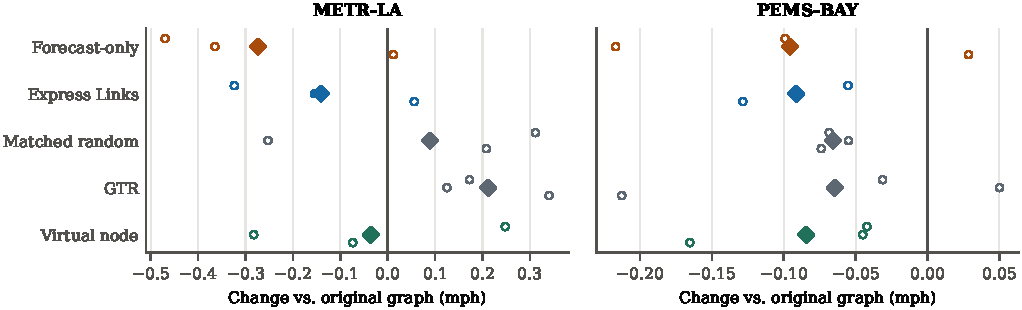
\includegraphics[width=.92\textwidth]{figs/replication_seeds.pdf}
\caption{\prev{Seed-level change in 60-minute low-speed MAE at the 25 shared roads relative to the original graph.}}
\label{fig:repseeds}
\end{figure*}

\subsection{Where the selected links sit}
\prev{The two ridge-based selectors placed their links very differently. Fig.~\ref{fig:map} draws the 25 links of Express Links, Forecast-only and matched random on the METR-LA road graph. Grey lines are road-graph edges, arrows are added links, and coloured dots mark their target roads. Express Links draws long links from three source roads in the north-west, while Forecast-only links are shorter and fan into the central corridor. The matched random links share the Express Links targets but take random eligible sources. The median Express Links pair was eight hops apart on METR-LA and seven on PEMS-BAY, against five on both datasets for Forecast-only. Relative to all eligible pairs, the median resistance percentiles were 88.6 for Express Links and 14.0 for Forecast-only on METR-LA, and 94.4 and 41.7 on PEMS-BAY. The two selectors shared 21 of 25 destinations on METR-LA and 12 of 25 on PEMS-BAY.}

\begin{figure*}[!t]
\centering
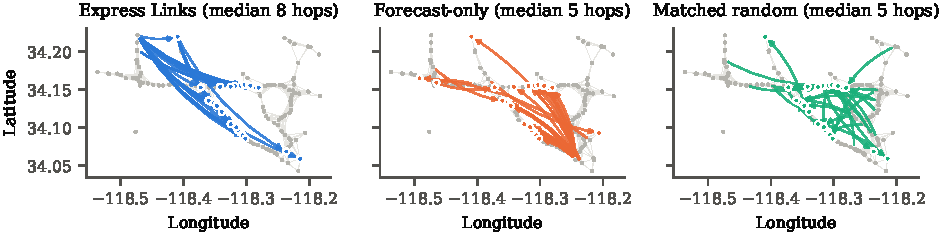
\includegraphics[width=\textwidth]{figs/links_map.pdf}
\caption{\prev{The 25 directed links added to the METR-LA road graph by Express Links, Forecast-only and matched random selection.}}
\label{fig:map}
\end{figure*}

\prev{Fig.~\ref{fig:linkprops} compares the chosen links one by one. Panel (a) gives the effective resistance of each chosen pair in the original graph, and panel (b) gives the held-out ridge gain for Express Links and Forecast-only; the archived GTR and random outputs have no comparable gain scores. Black bars mark medians. The median pair resistance was 5.81 on METR-LA and 4.20 on PEMS-BAY for Express Links, close to GTR (6.06 and 3.77). Forecast-only chose better-connected pairs (1.40 and 2.27), closer to matched random (1.65 and 2.86), and its links had higher median ridge gains (1.00 against 0.53\ms{} on METR-LA, and 0.87 against 0.60\ms{} on PEMS-BAY). Because the random graph shared the Express Links destinations while Forecast-only could link to other roads, these comparisons reflect both the choice of source and where the links were added.}

\begin{figure}[!t]
\centering
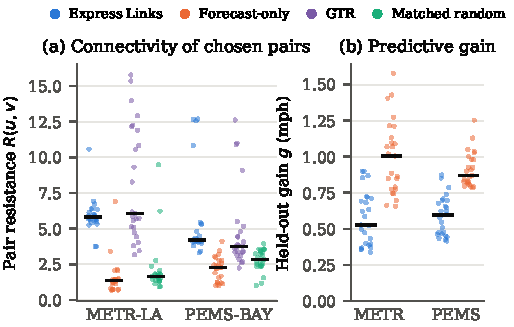
\includegraphics[width=\columnwidth]{figs/link_properties.pdf}
\caption{\prev{Pair resistance and held-out ridge gain of the links chosen by each selector.}}
\label{fig:linkprops}
\end{figure}

\subsection{E4 and E5: Over-squashing diagnostics}
\prev{The two diagnostics ask whether the trained models actually used the selected source roads more, as over-squashing relief would predict. Table~\ref{tab:diag} lists each rule and its outcome. The week-swap test (D1) found that Express Links increased source use beyond random, with an interval above zero, on only one of three seeds. We also asked whether the original Graph WaveNet used weakly connected sources less than better-connected ones. Across 9{,}626 matched pairs, none of the three seeds met the rule, and the same-target and low-speed versions of the check agreed. One caveat applies to the primary D1 test: the links in the two graphs came from different pair sets with different resistance distributions, so the choice of random control affects how the result can be read.}

\begin{table}[!t]
\centering
\caption{\prev{Outcomes of the over-squashing diagnostics on METR-LA Graph WaveNet checkpoints (seeds 0--2).}}
\label{tab:diag}
\footnotesize
\setlength{\tabcolsep}{3pt}
\begin{tabular}{@{}p{4.3cm}p{3.6cm}@{}}
\toprule
Rule & Outcome \\
\midrule
\multicolumn{2}{@{}l}{\textit{D1: week-swap diagnostic}}\\
Secondary: original model uses low-$R$ sources more than matched high-$R$ sources (9{,}626 pairs) & not supported, 0/3 seeds \\
\quad same target road & not supported, 0/3 \\
\quad low-speed readings only & not supported, 0/3 \\
Primary: EL adds use beyond random ($A-B>0$) & not supported, 1/3 seeds \\
\midrule
\multicolumn{2}{@{}l}{\textit{D2: five-donor diagnostic}}\\
Added reliance, EL vs.\ original & $+0.0210$ [$-0.0057$, $+0.0486$] \\
Added reliance, EL vs.\ random & $+0.0224$ [$+0.0041$, $+0.0426$] \\
Seeds above $+0.01$\ms{} (each contrast) & 3/3 \\
Gate (both lower bounds $>{+}0.01$) & not passed; follow-up not run \\
\bottomrule
\end{tabular}
\end{table}

\prev{The five-donor test (D2) covered 27{,}439 low-speed readings at the 25 roads over 21 test days. All nine checkpoints reproduced their saved forecasts exactly before we swapped any inputs. Express Links increased reliance on its sources by 0.0210\ms{} compared with the original graph and by 0.0224\ms{} compared with matched random links. Every seed cleared the 0.01\ms{} margin in both comparisons, but the lower interval bounds were $-0.0057$ and $+0.0041$\ms{}. The rule required both bounds to exceed 0.01\ms{}, so the planned high- versus low-resistance follow-up was not run. Fig.~\ref{fig:mechanism} plots both diagnostics with their intervals: D1 needed support above zero on two of three seeds, and D2 needed both pooled lower bounds above 0.01\ms{} as well as its seed condition.}

\begin{figure*}[!t]
\centering
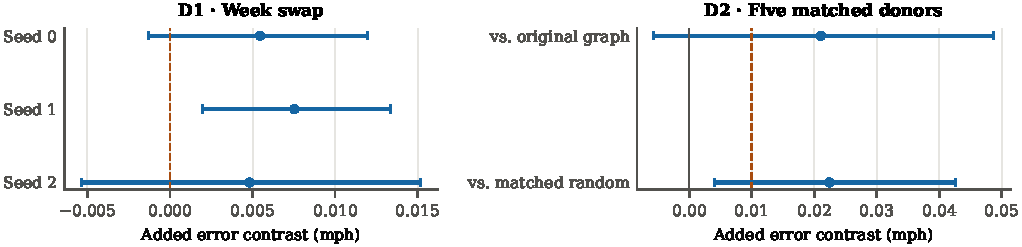
\includegraphics[width=.87\textwidth]{figs/mechanism.pdf}
\caption{\prev{Input-replacement contrasts and 95\% day-bootstrap intervals for the two diagnostics on METR-LA.}}
\label{fig:mechanism}
\end{figure*}

\subsection{E6: Transfer to DCRNN}
\prev{The DCRNN baseline behaved as expected. With the original graph, its three runs averaged 2.685, 3.073 and 3.529\ms{} at 15, 30 and 60 minutes, close to the published DCRNN values of 2.77, 3.15 and 3.60\ms{} \cite{li2018dcrnn,wu2019graphwavenet}. We then trained DCRNN on four of the frozen METR-LA graphs, which were also used with Graph WaveNet in Table~\ref{tab:sixway}. Table~\ref{tab:dcrnn} gives the 60-minute MAE at the shared 25 roads and across all roads, for low-speed and all readings.}

\begin{table}[!t]
\centering
\caption{\prev{DCRNN transfer on METR-LA: 60-minute MAE (mph), mean over seeds 0--2.}}
\label{tab:dcrnn}
\footnotesize
\setlength{\tabcolsep}{3.5pt}
\begin{tabular}{@{}lrrrr@{}}
\toprule
& \multicolumn{2}{c}{Shared 25 roads} & \multicolumn{2}{c}{All roads} \\
\cmidrule(lr){2-3}\cmidrule(lr){4-5}
Graph & Low speed & All speeds & Low speed & All speeds \\
\midrule
Original & 8.383 & 3.122 & 7.747 & 3.529 \\
Ridge Express Links & 8.326 & 3.100 & 7.752 & 3.517 \\
Forecast-only & \best{8.051} & \best{3.076} & 7.760 & 3.526 \\
Matched random & 8.270 & 3.102 & \best{7.714} & \best{3.513} \\
\bottomrule
\end{tabular}
\end{table}

\prev{With DCRNN, Forecast-only again had the lowest low-speed MAE at the shared roads (8.051\ms{}, against 8.383 for the original graph and 8.270 for matched random). It beat random links on every seed, by 0.160, 0.294 and 0.205\ms{}, and so met the transfer rule. Ridge-based Express Links also met the rule, since it beat random on two seeds and had a lower mean than the original graph, although its mean stayed above random's. Across the whole network the picture was different: Forecast-only lowered low-speed error with Graph WaveNet but raised it slightly with DCRNN. Fig.~\ref{fig:twomodels} puts the two models side by side. On the primary metric (a), Forecast-only gives the largest reduction in both models. Its network-wide low-speed gain (b) appears only in Graph WaveNet. Overall error (c) changes by at most about 0.015\ms{} for any graph. The clearest evidence of transfer is therefore at the shared target roads.}

\begin{figure*}[!t]
\centering
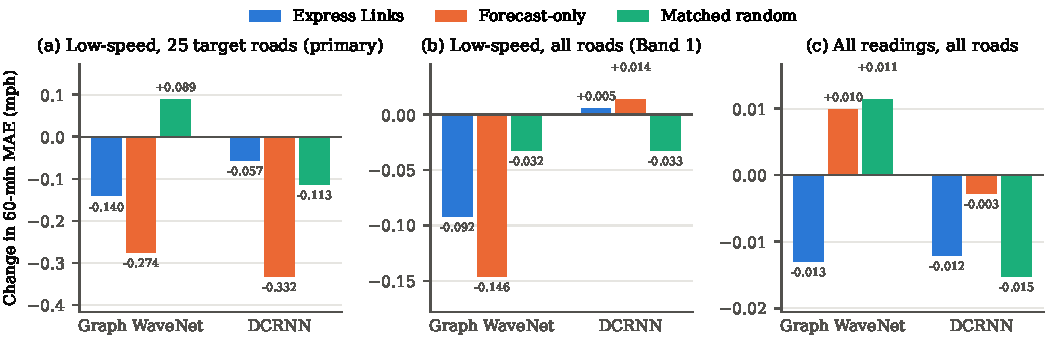
\includegraphics[width=\textwidth]{figs/two_models.pdf}
\caption{\prev{Change in 60-minute MAE relative to the original graph for the same frozen links in Graph WaveNet and DCRNN (METR-LA, mean of three seeds).}}
\label{fig:twomodels}
\end{figure*}

\prev{\textit{Supplementary check with DCGRU.} Before we switched to the published DCRNN code, our diagnostic script had also trained a simpler DCRNN-style model that we wrote ourselves (DCGRU) on the same frozen graphs, seeds and test readings. We did not look at these results until after the switch, and the plan we wrote at the switch committed us to reporting them as a supplementary check. Forecast-only again had the lowest low-speed MAE at the shared roads (8.157\ms{}, against 8.348 for the original graph) and beat matched random links on all three seeds ($-0.253$, $-0.783$ and $-0.048$\ms{}), so the transfer rule held. Ridge-based Express Links beat random on two seeds, but its mean (8.497\ms{}) was above the original graph's, so it failed the rule. Random links did not help DCGRU (8.519\ms{}). Forecast-only also had the lowest Band~1 error across all roads (7.773 against 7.935\ms{}), while overall 60-minute MAE varied by less than 0.02\ms{} across the four graphs. Table~\ref{tab:second_models} in Appendix~\ref{app:other} lists the full DCRNN and DCGRU results.}

\subsection{E7: Tuning Forecast-only}\label{sec:tuning}
\prev{\textit{Grid.} We first varied the link budget and the minimum hop distance at the original link weight, using validation data and seeds 0 and 1. Fig.~\ref{fig:grid} shows each set-up as the change in 60-minute MAE from current Forecast-only (the boxed cell: at least 3 hops, 25 links). Panel (a) gives Band~1 error over all roads, which is the tuning metric, and panel (b) gives overall error. All twelve set-ups passed the overall-error limit. Only one improved on current Forecast-only in Band~1: allowing one-hop links at 25 links gave $-0.011$\ms{}, short of the 0.02\ms{} threshold. Larger budgets generally reduced overall error, by up to 0.049\ms{} at 100 links and three hops, but raised Band~1 error by 0.06 to 0.26\ms{}. With only 10 links, Band~1 error was worse at every distance. The original graph was 0.136\ms{} worse than current Forecast-only on this metric.}

\begin{figure*}[!t]
\centering
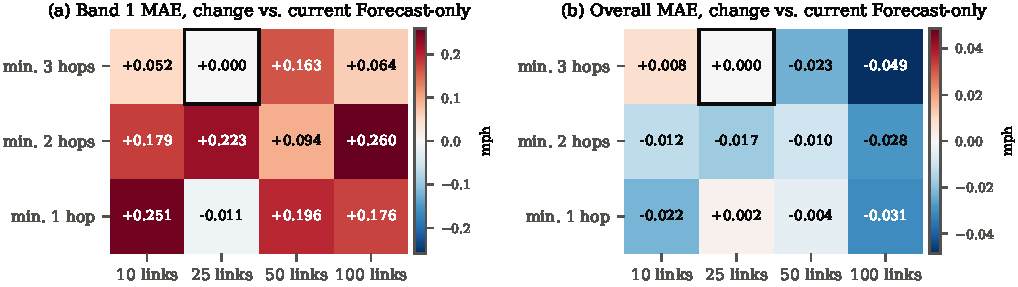
\includegraphics[width=0.92\textwidth]{figs/tuning_grid.pdf}
\caption{\prev{Validation grid of link budget and minimum hop distance for Forecast-only on METR-LA.}}
\label{fig:grid}
\end{figure*}

\prev{\textit{Weights and allocation.} Next we tried half and double link weights and allowed more than one link per road. Table~\ref{tab:tuneval} lists the main set-ups. The upper block averages seeds 0 and 1 and was used for selection; the lower block repeats the leading set-ups with seeds 0 to 4. Each $\Delta$ is against current Forecast-only (at least 3 hops, 25 links, $1\times$ weight), and bold marks the best value per block and column. Half-weight links with a one-hop minimum gave the lowest validation Band~1 error, $-0.051$\ms{} against current Forecast-only, with slightly lower overall error. This passed both thresholds and became the candidate. Doubling the weight increased Band~1 error for both hop settings, and halving the weight of the three-hop set-up also increased it ($+0.233$\ms{}). The inner model used for error-based allocation had enough low-speed readings on 205 of 207 roads. Allowing up to three links per road raised Band~1 error by 0.086\ms{} when links were allocated by gain and by 0.119\ms{} when they were allocated by error. The test candidate therefore kept one link per target road, with 25 links, a one-hop minimum and half weight.}

\begin{table}[!t]
\centering
\caption{\prev{Forecast-only tuning on METR-LA validation data: 60-minute MAE (mph) of the main set-ups.}}
\label{tab:tuneval}
\footnotesize
\setlength{\tabcolsep}{2.4pt}
\begin{tabular}{@{}lccc@{}}
\toprule
Set-up (min.\ hops, links, weight) & Band 1 ($\Delta$) & Overall ($\Delta$) & 25 roads \\
\midrule
\multicolumn{4}{@{}l}{\textit{Selection, seeds 0--1}}\\
1, 25, $0.5\times$ (winner) & \best{7.346} ($-$0.051) & 3.237 ($-$0.012) & 7.653 \\
1, 25, $1\times$ & 7.386 ($-$0.011) & 3.251 ($+$0.002) & 7.890 \\
3, 25, $1\times$ (current FO) & 7.397 & 3.249 & \best{7.570} \\
3, 100, $1\times$ & 7.461 ($+$0.064) & \best{3.200} ($-$0.049) & 7.797 \\
3, 25, $2\times$ & 7.488 ($+$0.091) & 3.230 ($-$0.019) & 7.928 \\
1, 25, $2\times$ & 7.502 ($+$0.105) & 3.221 ($-$0.028) & 7.760 \\
3, 25, $0.5\times$ & 7.630 ($+$0.233) & 3.216 ($-$0.033) & 8.216 \\
Up to 3 per road, by gain & 7.482 ($+$0.086) & 3.233 ($-$0.016) & 7.932 \\
Up to 3 per road, by error & 7.516 ($+$0.119) & 3.234 ($-$0.014) & 8.089 \\
Original graph & 7.532 ($+$0.136) & 3.241 ($-$0.008) & 8.084 \\
\midrule
\multicolumn{4}{@{}l}{\textit{Confirmation, seeds 0--4}}\\
Current FO & \best{7.474} & 3.243 & 7.884 \\
Tuned (1, 25, $0.5\times$) & 7.491 ($+$0.017) & \best{3.237} ($-$0.006) & \best{7.842} \\
Original graph & 7.581 ($+$0.107) & 3.240 ($-$0.002) & 8.036 \\
Random, matched to tuned & 7.594 ($+$0.120) & 3.241 ($-$0.001) & 8.136 \\
\bottomrule
\end{tabular}
\end{table}

\prev{\textit{Five-seed check.} Adding seeds 2 to 4 changed the validation ranking. Over all five seeds, the tuned graph's Band~1 MAE was 7.491\ms{}, against 7.474 for current Forecast-only, 7.581 for the original graph and 7.594 for the tuned graph's matched random control.}

\prev{\textit{Final test.} Following the locked plan, we then scored the tuned graph once on the METR-LA test split, which had already been used earlier in the project. Table~\ref{tab:final} gives the mean 60-minute MAE over seeds 0 to 4; Band~1 is the primary metric for the tuning study and covers low-speed readings on all roads. Tuning lowered Band~1 MAE relative to the original graph by 0.0809\ms{} (95\% day interval $-0.1112$ to $-0.0526$) and relative to matched random by 0.1014\ms{} ($-0.1293$ to $-0.0746$), with intervals over 24 test days. Current Forecast-only was still better on this metric, at 7.4854\ms{} against 7.5285\ms{} for the tuned graph, a paired difference of $+0.0431$\ms{} ($+0.0211$ to $+0.0681$). Tuning gave slightly lower overall MAE (3.5470 against 3.5575\ms{}, difference $-0.0105$, interval $-0.0205$ to $+0.0006$). At the 25 original target roads, the low-speed difference was $-0.0145$\ms{}, with an interval of $-0.0853$ to $+0.0529$.}

\begin{table}[!t]
\centering
\caption{\prev{Locked METR-LA tuning test: mean 60-minute MAE (mph) over seeds 0--4.}}
\label{tab:final}
\footnotesize
\setlength{\tabcolsep}{4.5pt}
\begin{tabular}{@{}lrrr@{}}
\toprule
Graph & Band 1 & Overall & Low speed, 25 roads \\
\midrule
Original graph & 7.6094 & 3.5508 & 7.9911 \\
Current Forecast-only & \best{7.4854} & 3.5575 & 7.8757 \\
Tuned Forecast-only & 7.5285 & \best{3.5470} & \best{7.8612} \\
Random, matched to tuned & 7.6300 & 3.5487 & 8.1391 \\
\bottomrule
\end{tabular}
\end{table}

\prev{Fig.~\ref{fig:final} shows these paired differences with their intervals. For Band~1 (orange), the intervals favour the tuned graph over the original and random graphs, and favour current Forecast-only over the tuned graph. Because the tuned graph missed the primary rule, we kept the original Forecast-only configuration of 25 links, a three-hop minimum and median weight, and did not run the planned DCRNN transfer on PEMS-BAY. Over five seeds on the same test split, current Forecast-only beat the original graph by 0.124\ms{} on the primary metric.}

\begin{figure}[!t]
\centering
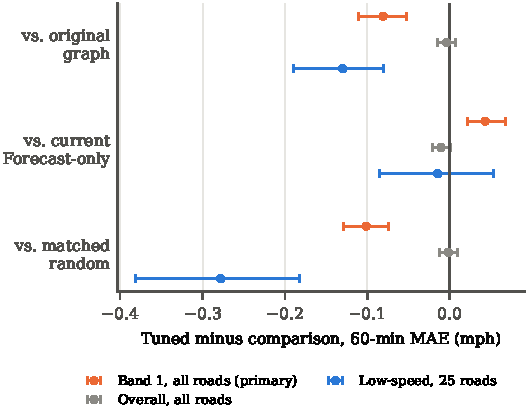
\includegraphics[width=0.92\columnwidth]{figs/final_test.pdf}
\caption{\prev{Paired test differences for the tuned Forecast-only set-up, with 95\% day-bootstrap intervals (METR-LA, seeds 0--4).}}
\label{fig:final}
\end{figure}

%======================================================================
\section{Discussion}\label{sec:discussion}
%======================================================================

\subsection{What improves with sparse links}
\prev{No single graph was best on every metric. On METR-LA, Forecast-only reduced error on slow readings at the shared target roads with both Graph WaveNet and DCRNN, and it did so on every seed when compared with matched random links. On PEMS-BAY its low-speed error at those roads was almost the same as that of ridge-based Express Links. When we scored all roads and all speeds at 60 minutes, the virtual node was best on both datasets in the six-way comparison, but it used a much larger edge budget than the sparse selectors. The gains on slow traffic were also larger than the changes in overall error, which stayed within a few hundredths of a mph for every graph. A study that reported only overall MAE would have missed most of the differences between the selectors.}

\subsection{What the diagnostics establish}
\prev{Our original motivation was to give distant information a way around bottlenecks. The evidence for that mechanism is weak. In the METR-LA bottleneck subset, all seven Stage~1 graphs missed the hour-ahead jam warnings under the original event rule. In the follow-up, the selector with the lowest target-road error, Forecast-only, chose pairs that were closer and better connected on average, which is the opposite of what bottleneck relief would suggest. The week-swap test gave no support for the idea that the original model under-used weakly connected sources. In the five-donor test, the estimated reliance on the selected sources did increase, but the lower interval bounds fell short of the margin we set in advance. A network with stronger bottlenecks and useful signals on both sides would allow a more direct test of the original idea.}

\prev{Our findings agree with recent work that questions how much rewiring helps on real data. A re-evaluation of curvature-based rewiring on standard node-classification benchmarks found that many reported gains came from favourable hyperparameter settings rather than consistent improvements, and that the edges chosen as bottlenecks often did not meet the bottleneck condition the methods assume \cite{tori2025revisited}. A recent survey of rewiring methods makes a related recommendation: studies should show that the task depends on information beyond a small neighbourhood, check gains against matched-budget random controls and report the edit budget \cite{attali2026survey}. Our study followed that design, with a fixed budget of 25 links, matched random links and several seeds. Under those controls, Forecast-only achieved the lowest mean low-speed MAE on the shared evaluation roads, while resistance reduction alone did not reliably predict forecasting gains.}

\section{Limitations and Future Work}\label{sec:limitations}
\subsection{Limitations}
\rev{\textbf{Data and seeds.} We tested on two highway datasets, and the architecture transfer and the input-replacement diagnostics were limited to METR-LA. Most comparisons used three training seeds, so the mean errors rest on a small sample of training runs, and the seed spread was often as large as the differences between graphs. The half-weight configuration led after two validation seeds, then lost that lead at five seeds and on test. The day-bootstrap intervals describe variation across test days for the fitted models; they do not include variation from retraining.}

\rev{\textbf{Test-split reuse.} The METR-LA test split had already been used earlier in the project, so the tuning test is a single planned look at data we had seen before rather than a fully independent test.}

\rev{\textbf{Destination mismatch.} We scored all methods on the same readings, but the selectors did not always add links to the same destinations. We also chose the evaluation metric after the pilot and based it on the roads that received an Express Links edge, so the shared evaluation roads favour that selector's destinations.}

\subsection{Future research directions}
\rev{\textbf{Fixed-destination test.} A follow-up could fix the destinations, draw several random graphs and match the controls on hop distance. This would show how much the choice of source contributes on its own.}

\rev{\textbf{Bottleneck benchmark.} METR-LA has only 9 sensors behind its screened bottleneck and PEMS-BAY has none. A direct test of the over-squashing mechanism needs a held-out benchmark with verified bottleneck coverage, such as a region of LargeST \cite{liu2023largest}.}

\rev{\textbf{More seeds and models.} Running five or more seeds for every comparison, and repeating the transfer test with DCRNN and other forecasters on PEMS-BAY, would show whether the low-speed gains of Forecast-only hold beyond METR-LA and Graph WaveNet.}

\section{Conclusion}\label{sec:conclusion}
\prev{We asked which 25 extra sensor links help a graph forecaster predict slow traffic an hour ahead, and whether links chosen to relieve over-squashing do better than links chosen for their forecasting value. We tested this in two stages on METR-LA and PEMS-BAY, with Graph WaveNet as the main forecaster and DCRNN as a second architecture.}

\prev{The first stage tested the selector we originally proposed, which balances lead--lag correlation against the drop in effective resistance. Its gains were small. Overall 60-minute MAE fell by about 0.01\ms{} on both datasets, which on METR-LA was within the seed-to-seed spread, and no graph produced useful hour-ahead jam warnings behind the METR-LA bottleneck. Larger resistance reductions did not guarantee larger forecasting gains: random links lowered total resistance by more than a third on METR-LA and still left the error slightly higher.}

\prev{The second stage scored each link by how much its source improved a held-out ridge forecast of its target. Forecast-only, which ranks links by this gain alone, gave the lowest mean error on low-speed readings at the shared evaluation roads on both datasets. On METR-LA it reduced that error by 0.274\ms{} relative to the original graph and beat matched random links on every seed. The result carried over to DCRNN, where Forecast-only again had the lowest error on those readings and beat random links on all three seeds. Tuning the link budget, hop distance and link weight did not improve on the original Forecast-only configuration, which stayed 0.124\ms{} better than the original graph on the locked test.}

\prev{The over-squashing explanation found little support. Forecast-only chose short, well-connected links rather than links across bottlenecks. The week-swap test found no sign that the original model under-used weakly connected sources, and the five-donor test found more reliance on the Express Links sources but not by the margin we set in advance. The virtual node, which adds one hub linked to every sensor, gave the lowest overall MAE in the six-way comparison, but at a much larger edge budget.}

\prev{Taken together, the results suggest that a few links chosen for their measured forecasting value help most where errors are largest, on slow traffic at the shared evaluation roads, while their effect on overall error is small. Reporting errors by speed band, and comparing against matched random links over several seeds, was necessary to see this. This is in line with recent studies that find rewiring for over-squashing gives smaller and less consistent gains on real data than theory suggests. Whether relieving over-squashing adds anything beyond forecasting value remains open, and a test on a network with clear bottlenecks would be the natural next step.}

\section*{Data Availability}
\rev{The code, run-level results, frozen link graphs, decision records and figure scripts for this study are available at \url{https://github.com/alzahraa77/express-links-mlr570}. The repository README links each table and figure in this report to the script and saved record behind it. METR-LA and PEMS-BAY are public benchmarks \cite{li2018dcrnn}; the scripts download them automatically. Appendices~\ref{app:horizon} and~\ref{app:other} give the results by forecast horizon, the jam-warning scores and the supplementary model comparisons.}

\bibliographystyle{IEEEtran}
\bibliography{refs}

\FloatBarrier
\onecolumn
\appendices
\section{Forecasting results by horizon}\label{app:horizon}
\prev{Table~\ref{tab:horizons} gives the six-way Graph WaveNet results on all observed test readings at 15, 30 and 60 minutes, together with the average over the 12 horizons. Each entry is MAE / RMSE / MAPE (mph, mph, percent), averaged over three seeds. Fig.~\ref{fig:horizon_extra} shows the network-wide MAE difference from the original graph at every horizon, with all panels on the same vertical scale; negative values favour the added links. Together they give a network-wide view to set beside the low-speed results in Table~\ref{tab:sixway}.}
\begin{table}[H]
\centering
\small
\caption{\rev{Six-way Graph WaveNet comparison on all observed test readings by forecast horizon.}}
\label{tab:horizons}
\begin{tabular}{@{}llrrrr@{}}
\toprule
Dataset & Graph & 15 minutes & 30 minutes & 60 minutes & 12-horizon mean \\
\midrule
METR-LA & Original & 2.708 / 5.164 / 7.01 & 3.096 / 6.208 / 8.50 & 3.554 / 7.331 / 10.19 & 3.058 / 6.074 / 8.35 \\
 & Ridge Express Links & 2.698 / 5.156 / 6.93 & 3.079 / 6.181 / 8.40 & 3.541 / 7.300 / 10.09 & 3.043 / 6.052 / 8.26 \\
 & Forecast-only & 2.703 / 5.155 / 6.93 & 3.087 / 6.185 / 8.35 & 3.564 / 7.339 / 10.01 & 3.055 / 6.065 / 8.21 \\
 & GTR & 2.699 / 5.150 / 6.97 & 3.083 / 6.179 / 8.48 & 3.542 / 7.316 / 10.31 & 3.046 / 6.056 / 8.36 \\
 & Matched random & 2.713 / 5.177 / 6.98 & 3.103 / 6.214 / 8.46 & 3.565 / 7.355 / 10.17 & 3.066 / 6.092 / 8.32 \\
 & Virtual node & 2.698 / 5.153 / 6.98 & 3.080 / 6.175 / 8.46 & 3.522 / 7.270 / 10.09 & 3.039 / 6.040 / 8.31 \\
PEMS-BAY & Original & 1.316 / 2.758 / 2.75 & 1.653 / 3.739 / 3.75 & 1.968 / 4.565 / 4.74 & 1.592 / 3.552 / 3.61 \\
 & Ridge Express Links & 1.314 / 2.752 / 2.76 & 1.651 / 3.739 / 3.74 & 1.963 / 4.557 / 4.71 & 1.590 / 3.549 / 3.61 \\
 & Forecast-only & 1.318 / 2.762 / 2.75 & 1.651 / 3.732 / 3.71 & 1.964 / 4.548 / 4.69 & 1.591 / 3.545 / 3.59 \\
 & GTR & 1.314 / 2.753 / 2.75 & 1.649 / 3.730 / 3.74 & 1.955 / 4.534 / 4.71 & 1.586 / 3.537 / 3.60 \\
 & Matched random & 1.317 / 2.758 / 2.76 & 1.652 / 3.735 / 3.74 & 1.966 / 4.556 / 4.71 & 1.591 / 3.549 / 3.61 \\
 & Virtual node & 1.310 / 2.739 / 2.73 & 1.641 / 3.692 / 3.68 & 1.948 / 4.484 / 4.63 & 1.580 / 3.503 / 3.55 \\
\bottomrule
\end{tabular}
\end{table}

\begin{figure}[H]
\centering
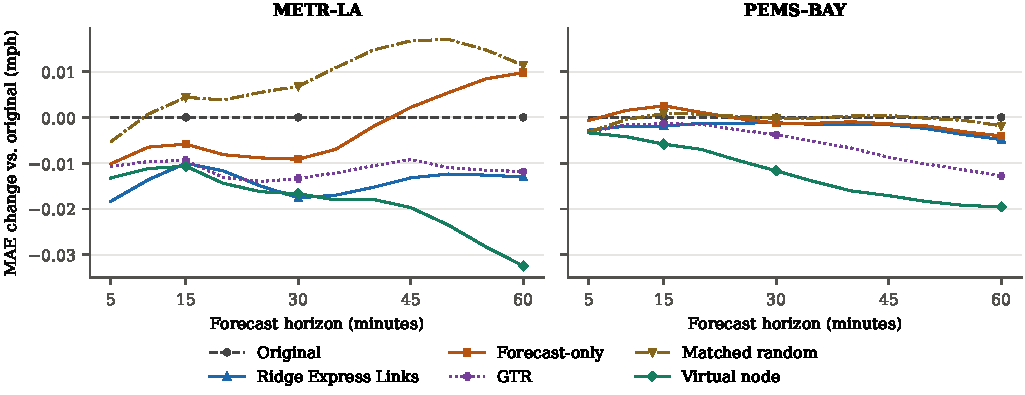
\includegraphics[width=.83\textwidth]{figs/horizon_profiles.pdf}
\caption{\prev{Network-wide MAE difference from the original graph at each forecast horizon (seeds 0--2).}}
\label{fig:horizon_extra}
\end{figure}

\clearpage
\section{Additional event and architecture results}\label{app:other}
\prev{Table~\ref{tab:events} gives the jam-warning recall and precision on all roads from the Stage~1 study, averaged over three seeds. Here a warning must predict a jam onset under the original event rule, unlike the PEMS-BAY tolerance check in Section~\ref{sec:stage1}, which measures speed error at events that did occur. Table~\ref{tab:second_models} gives the DCRNN and DCGRU results on METR-LA as mean MAE over three seeds: low-speed error at the shared target roads, Band~1 error on all roads, and overall error on all observed speeds.} The source package also contains the exploratory LargeST runs. The one-seed flow pilot and the separate hub-count sweep use different forecasting setups and their own distance or original-graph references.
\begin{table}[H]
\centering
\small
\caption{\rev{Stage~1 jam-warning recall and precision (percent) on all roads.}}
\label{tab:events}
\begin{tabular}{@{}llrrrr@{}}
\toprule
Dataset & Graph & Recall at 30 min & Precision at 30 min & Recall at 60 min & Precision at 60 min \\
\midrule
METR-LA & Original & 19.72 & 57.15 & 7.70 & 56.04 \\
 & Random & 19.80 & 55.30 & 7.78 & 56.27 \\
 & Resistance only & 20.19 & 55.71 & 8.61 & 58.94 \\
 & Correlation only & 19.18 & 57.31 & 9.05 & 58.27 \\
 & Same-side & 20.50 & 55.09 & 8.19 & 54.44 \\
 & Greedy lead--lag & 20.21 & 54.53 & 8.59 & 58.01 \\
 & Virtual node & 19.80 & 59.96 & 8.07 & 58.20 \\
PEMS-BAY & Original & 24.74 & 61.85 & 2.00 & 42.02 \\
 & Random & 22.45 & 61.58 & 1.52 & 40.10 \\
 & Resistance only & 24.19 & 62.74 & 1.67 & 48.01 \\
 & Correlation only & 25.34 & 62.61 & 2.19 & 47.57 \\
 & Same-side & 24.04 & 62.21 & 1.73 & 44.77 \\
 & Greedy lead--lag & 23.41 & 62.22 & 3.03 & 48.60 \\
 & Virtual node & 26.31 & 64.06 & 1.93 & 53.05 \\
\bottomrule
\end{tabular}
\end{table}

\begin{table}[H]
\centering
\small
\caption{\rev{DCRNN and DCGRU results on METR-LA (MAE in mph, mean over seeds 0--2).}}
\label{tab:second_models}
\begin{tabular}{@{}llrrrr@{}}
\toprule
Model & Graph & 25 roads, low speed & Band 1 & Overall 60 min & Overall 12-horizon mean \\
\midrule
DCRNN & Original & 8.383 & 7.747 & 3.529 & 3.034 \\
 & Ridge Express Links & 8.326 & 7.752 & 3.517 & 3.029 \\
 & Forecast-only & 8.051 & 7.760 & 3.526 & 3.032 \\
 & Matched random & 8.270 & 7.714 & 3.513 & 3.028 \\
DCGRU & Original & 8.348 & 7.935 & 3.667 & 3.150 \\
 & Ridge Express Links & 8.497 & 7.978 & 3.677 & 3.156 \\
 & Forecast-only & 8.157 & 7.773 & 3.673 & 3.147 \\
 & Matched random & 8.519 & 7.992 & 3.659 & 3.141 \\
\bottomrule
\end{tabular}
\end{table}



\end{document}
